\documentclass[dissertation,math,vertlayout]{aaltoseries}
\graphicspath{{./Figures/}}

\usepackage[utf8]{inputenc}
\usepackage[english]{babel}
\usepackage{listings}
\usepackage{lipsum}
\usepackage{caption}
\usepackage{subcaption}
\usepackage{enumitem}
\usepackage{url}
\usepackage{amsmath}


\author{Pietro della Briotta Parolo}
\title{Analysis of cumulative and temporal patterns in science}
\begin{document}
%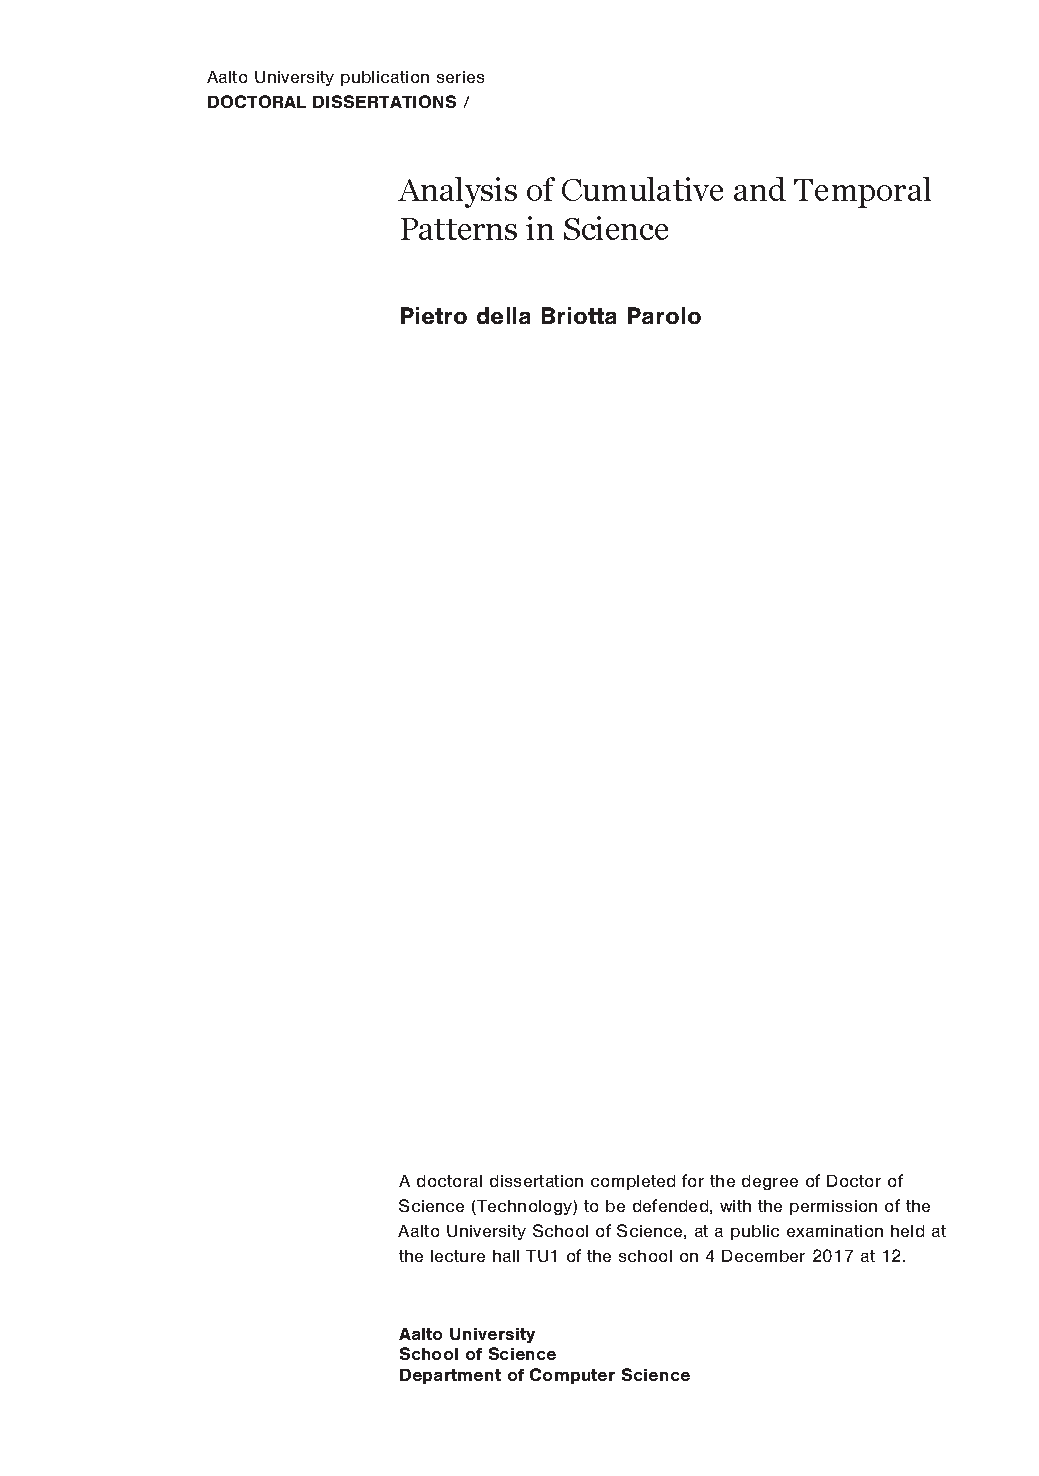
\includepdf[pages=-,pagecommand={},width=\textwidth]{Documents/header.pdf}



\begin{preface}[Espoo]

This thesis is the product of the work started at BECS in winter 2013 and eventually 
completed at the CS department in the summer of 2017. 

Looking back at these 4 years it's an interesting and exciting dive into
a lot of moments that have influenced heavily my life both privately as well as professionally.
Moving to Finland to pursue my academic passion was not just a big step forward in my career, but also
a big leap into a new world of which I admit I knew very little about beforehand. The first days were
therefore often as exciting as well as confusing and I need to thank the whole staff working at BECS
at the time for keeping an eye on me. In particular I'd like to mention Lauri Kovanen, who showed me 
the ways of the Python, Arnab Chatterjee and Marija Mitrovi\'c, with whom I often discussed about Science
in general, Raj Kumar Pan and Richard Darst, who had the patience to help me with often small
technical issues that I was not able to overcome on my own. Also, a huge thanks goes to my doctoral office mate, Darko Hric,
with whom I shared all the ups and downs of this adventure.

Leaving BECS was a huge change from many aspects. Most of the senior staff in the meantime had decided
to leave Aalto, ultimately leading to the departure also of my supervisor, Prof. Santo Fortunato,
whom I thank for guiding me and making me understand the pros and cons of life in academia. 
This period was extremely hectic, especially also with the organization of the iccss conference, which
unfortunately does not show up as part of this dissertation, but which is one of my proudest contribution
to Science, given the amount of work required and the quality of the final product, for which
Prof. Fortunato. This period culminated with yet another move to a new office within the CS department,
which represented the final stage of my stay at Aalto, now with the supervision
of Dr. Mikko Kivel\"a and Prof. Kimmo Kaski, to whom I owe a huge amount of gratitude
for "adopting" me in the final stage of my PhD and allowing me to conclude a project that turned out
to be both exciting and productive. Prof. Kaski was not only an excellent scientific
guide, but also a key figure in terms of supporting me, both personally and professionally,
until the very end of my experience at Aalto.

Finally, a big thanks to all those who have had the unfortunate experience
of being around me during my studies, but withouth whose support I wouldn't have been
able to get this far. 



\end{preface}



\clearpage
\tableofcontents
\listofpublications

\chapter{Introduction}

\section{Science of Science}
The underlying driving force of science has always been to start from empirical evidence in order to gain information
about the structure of the phenomena taking place around us. With such a pursuit in mind it was just a matter of time until science
would start investigating \textit{itself}. The moment came in the 60s, when the first bibliographic efforts required to improve the searchability of
scientific material took place in the form of a 
search for proper indexing \cite{bibliography_literature,Garfield108}
and therefore allowing, for the first time, to analyze the published material as its own data set. 
With only few previous works being carried out \cite{half_life}, the historical breakthrough in the field of science of science came with De Solla Price's work
\textit{Networks of Scientific Papers} \cite{deSollaPrice510}. De Solla's publication not only was one of the first 
to directly tackle the pattern of bibliographical references, but it also introduced key concepts for the development of the field,
starting from the need to analyze it in its topological structure as a network. Figs.\ref{fig:desolla_network} and \ref{fig:desolla_matrix}
show the earliest attempts of representing citation data as a network, even though the theory behind network science was still in its 
earliest stages. 



\begin{figure}[h!]
\centering
        \setbox0\hbox{%
                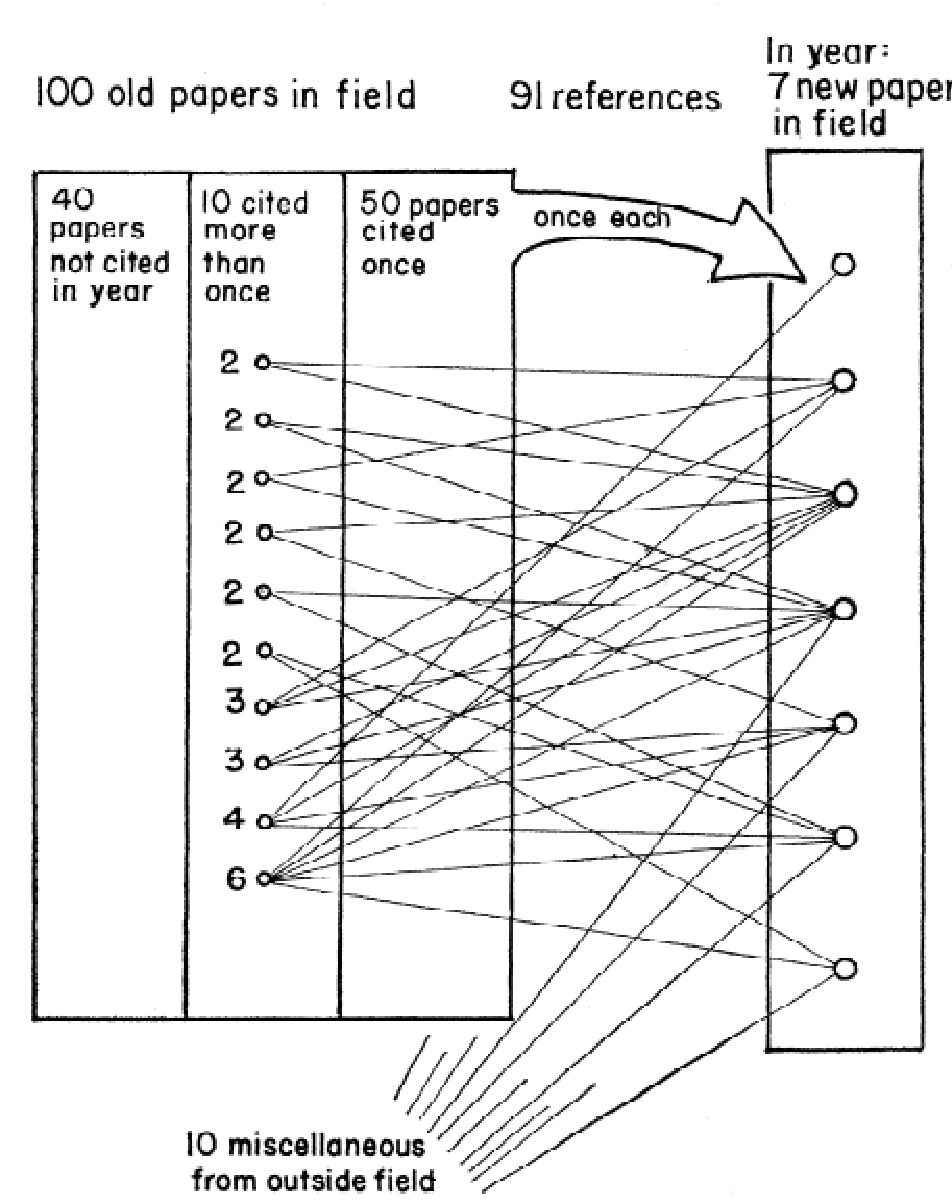
\includegraphics[width=.55\textwidth]{desolla.pdf}%
        }%
        \setbox2\hbox{%
                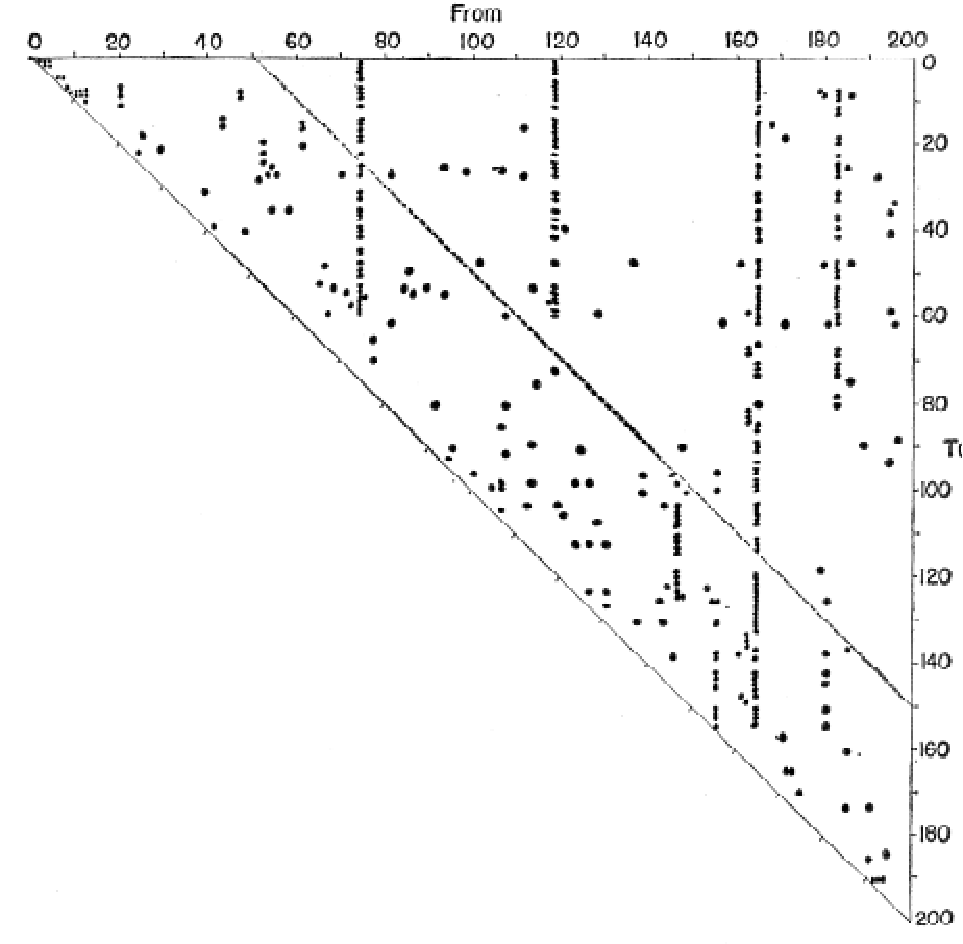
\includegraphics[width=.55\textwidth]{desollaadjacency.pdf}%
        }%
        \ifdim\ht0>\ht2
                \setbox0\hbox{%
                        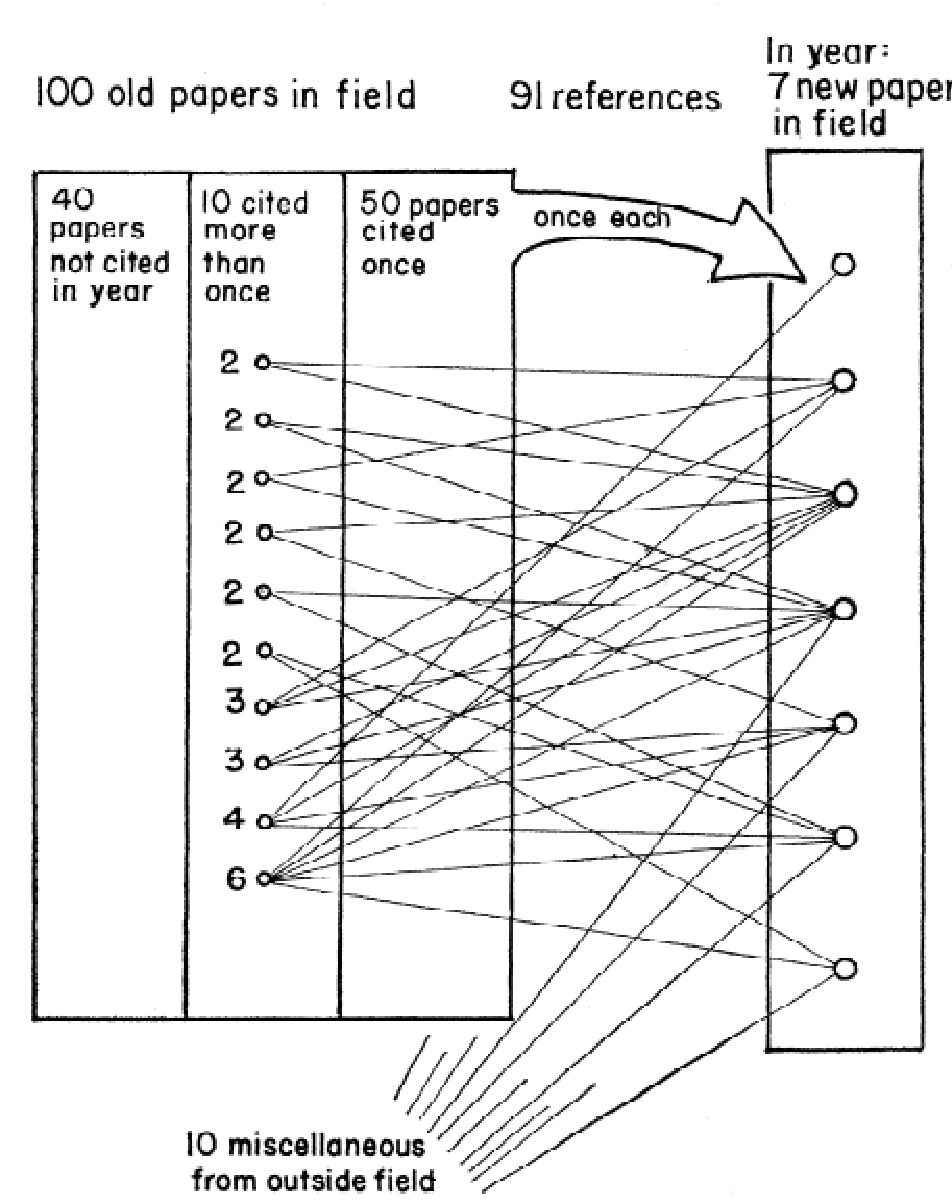
\includegraphics[height=\ht2]{desolla.pdf}%
                }%
        \else
                \setbox2\hbox{%
                        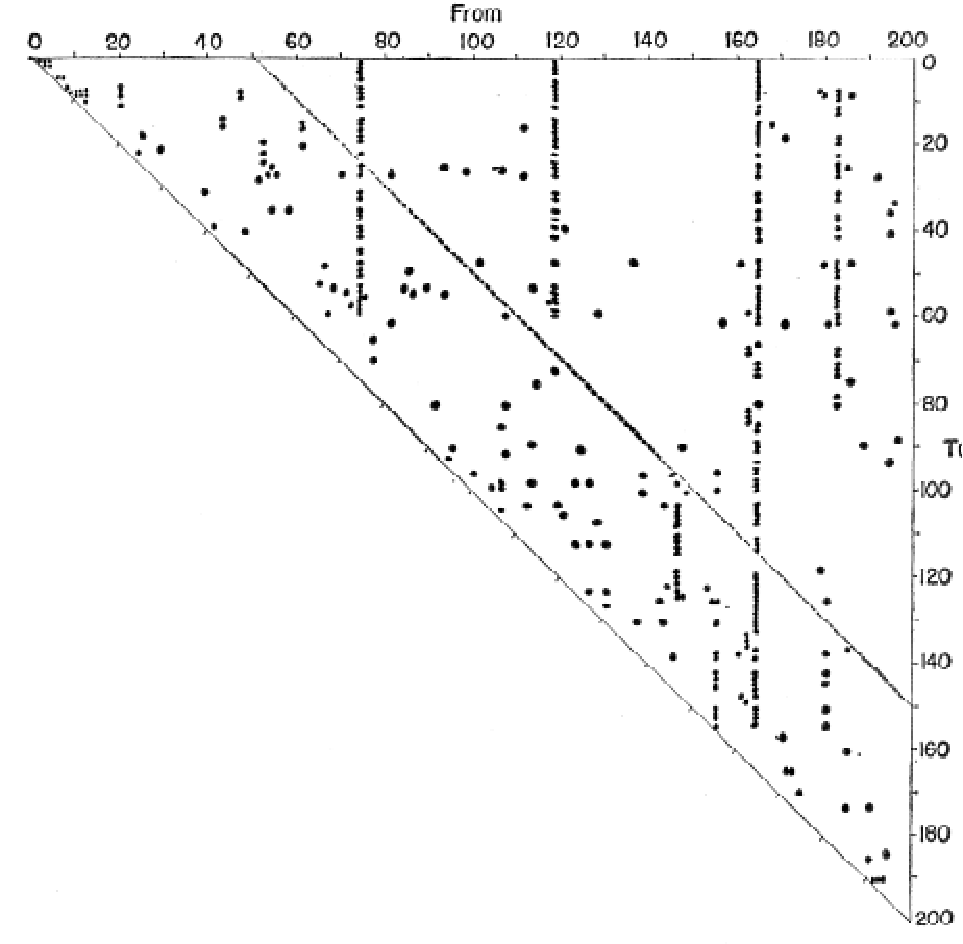
\includegraphics[height=\ht0]{desollaadjacency.pdf}%
                }%
        \fi
        \noindent
        \parbox{.45\textwidth}{%
                \centering
                \unhbox0
                \caption{Representation of citations as a network structure. Figure adapted from \cite{deSollaPrice510} with permission of The American Association for the Advancement of Science.}
                \label{fig:desolla_network}
        }%
        \hfil
        \parbox{.45\textwidth}{%
                \centering
                \unhbox2
                \caption{Representation of citations as an adjacency matrix. Figure adapted from \cite{deSollaPrice510} with permission of The American Association for the Advancement of Science.}
                \label{fig:desolla_matrix}
        }%
        
\end{figure}


What is most striking however, is that already in its origins, the study of the scientific production has required 
an analysis of science \textit{as a whole} and \textit{in time}. These key features are intrinsic properties of the entire
scientific production, since it is in the nature of science to build one's work on the top of previous ones, therefore adding a temporal dimension to
its development, as new discoveries and breakthroughs appear and link themselves to older ones. 
Since that seminal paper, the whole world, as well as the scientific one, has seen an amazing rise in technological possibilities,
which have affected heavily
the opportunities for collaborations, allowing people, as well as ideas, to move freely across the globe. 

These conditions, along with an improvement in
the economies in the post War era, has allowed science to grow at an amazing rate \cite{Larsen2010}. 
The amount of information generated by science has been growing exponentially at a rate close to a 4\% growth \textit{each year} in the last decades 
as shown in Fig.\ref{fig:growth_science}. Scientists are constantly dealing with the necessity to retrieve the latest results from their fields, which are also growing at
a fast rate; in such framework the ability to focus on the most relevant works becomes a key aspect. 
However, need for constant update requires to shift one's attention 
towards more recent scientific results, gradually discarding older ones. 

The same applies in the other direction, with scientists trying to get their latest publication known as much as possible, in order to gather \emph{attention} on their latest results. Therefore, scientists are actors in a market where the ability of reaching popularity in terms of scientific productivity has become a dominating aspect, implying that scientists/groups/institutions are all competing for attention in a market where the allocation thereof is structurally limited by one's ability to store information regarding all scientific results published in the past.


\begin{figure}[h!]
\centering
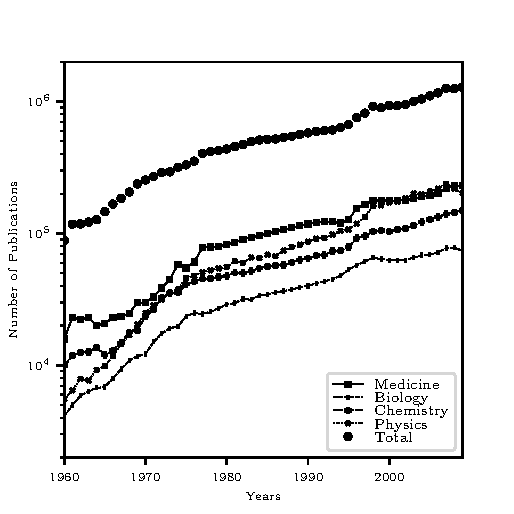
\includegraphics[width=.9\textwidth]{number_of_publications_thesis.pdf}%
\caption{Growth of publication in science and for a selected number of fields based on our ISI dataset of over 50 million publications and 600 million citations. The rate of growth can be well approximated by an exponential curve. Figure adapted from
Publication II.}\label{fig:growth_science}
\end{figure}

\section{Scope of the Thesis}
This thesis focus mainly on this temporal and cumulative aspect, investigating the changes that science has undergone in time due to its constantly changing nature.
Chapter \ref{Scientific Citations and Their Patterns} talks about the study of citation patterns, with their properties, biases and attempts at modeling them. Chapter \ref{Network Structure of Science} introduces the basic
concepts of network theory and how these concepts have been used to analyze the social and collaborative structure of science.
Chapter \ref{Science and Metrics} talks about the efforts in trying to determine the quality of scientific publications by the development of \textit{metrics}.
Finally, Chapter \ref{Results and Discussion} summarizes the content of Publications I-IV and discusses briefly how they contribute to the field of Science 
of Science.

\chapter{Scientific Citations and Their Patterns}\label{Scientific Citations and Their Patterns}
"\textit{If I have seen further, it is by standing on the shoulders of giants}''. This famous quote by Sir Isaac Newton summarizes perfectly the
moral obligation of a scientist to acknowledge the contribution of previous works to their own. Newton was perfectly aware that his
groundbreaking discoveries would have been impossible without the fundamental work done by previous scientists, from Aristotle to Galileo 
and Kepler, covering  centuries, if not millennia of scientific and philosophical endeavours.
While the recognition of the work done by predecessors at the times of Newton was done primarily by mentioning the names in the text or in private correspondence (as was the quote mentioned before) as a form of intellectual courtesy,
in modern times it has taken the form in scientific journals of a moral obligation based on an agreed voluntary scheme and is considered as a fundamental part of good scientific practice,
while for patents it even has a legal side, with previous patents being cited in order to be able to clarify how the new patent differs substantially from previously similar ones.
 Furthermore, due to the limited space available in a text, along 
  with the gradual process that turns recent discoveries into common knowledge, the publications mentioned in the reference lists represent
  an extremely careful and precise process of selection of a very limited number of works among thousands, if not millions, of related works published
  in recent times.
  
  As the results in aging literature are slowly assimilated as basic findings, scientists move on to newer results as the basis of their works,
  thus implicitly determining when a groundbreaking result becomes obsolete, as more impelling results require their attention. Just like Newton chose to acknowledge
  Galileo for a few selected results, but ignoring to do to the same with Pythagoras and his extensively used theorem, a recent paper in Quantum Physics will hardly
  mention any of the works of Einstein's Annus Mirabilis even though they are the very foundation on which its work is based on, since their results are now
  accepted as being universally known and do not need to be individually addressed anymore. 
  
It is for these reasons that ever since the early times of scientometrics, a lot of attention has been given to the analysis of the individual performance of
a single publication in terms of citations. A simple citation count is a superficial yet quantitative evaluation of the success of a paper and is deemed sufficient by some
to be able to compare and rank publications as well as scientists. However, the aforementioned process of obsolesce in science adds a dimension which has been described as
an \textit{attention economy} \cite{klamer_attention_2002} in which authors are aware that they have a limited amount of time to gather attention (i.e. citations)
and therefore compete against each other in order to obtain the maximum attention available. 

Such complex aspects that lead to the selection of the cited material has been the source of even more interest into the citation patterns as well as statistics of citation counts across
disciplines, countries and through time. This chapter will go through the most relevant works that have investigated the citation patterns in science, looking at the basic properties in citation
habits and with a summary of the most interesting attempts at modeling mathematically the citation patterns of scientists.



\section{Citation distributions} \label{sec:Citation Distributions}
 
One of the earliest questions that scientometrics tried to answer already with de Solla's seminal paper \cite{deSollaPrice510} has been: \textit{What is the functional form of the distributions of citations?}.
In particular, since the average value of citations gathered is bound to be structurally low as its value is linked to the finite number of 
references available, the interest was in the tail of the distributions, that is what are the citation values and patterns for the 
few exceptional publications capable to gather a number of citations that span over multiple orders of magnitude.
De Solla claimed, based on his limited data, that the functional form was power law like, with the number of papers with $c$ citations behaving like $N(c) \propto c^{-\alpha}$, with an estimate of $\alpha \in [2.5,3.6]$. 

For a long time, no one looked further into the claim with only Laherrère and Sornette in 1998 \cite{refId1} suggesting a generic stretched exponential form for the citation distribution
of \textit{authors}. It was only in 1998 that S. Redner tackled the topic in a systematic way \cite{refId0}. It is important to notice that such analysis was possible to be carried out
mainly thanks to the availability of a properly catalogued data set of scientific publications. By using two large data sets (~700 thousand papers obtained from the Institute for Scientific Information (ISI) and ~24 thousand papers
from Physical Review D) combining for more than 7 million citations, the author was able, for the first time, to carry out a thorough computational statistical analysis of citation
distributions. The results offered an interesting and, to a certain extent, worrisome insight of the relative popularity of scientific publications: almost half of the papers
failed to gather any citation at all from publication date to the time of the study, with $80\%$ of the publications gathering 10 citations or less. Even though also de Solla noticed a huge amount of uncited papers,
Redner was able to confirm the pattern also for a larger and more significant data set. The author concluded that a final evaluation of the functional form of the citation distribution
cannot be thoroughly computed as the tail of the distribution has not reached its final state, as the highly cited papers are still gathering citations. He also pointed out how a few 
highly cited papers can affect the higher-order moments of the distributions, thus making the task even harder. However, Redner succeeded in gathering some indirect measurement through
a Zipf plot \cite{Zipf}, providing evidence of a power law behaviour with $\alpha \approx 3$, compatible with de Solla's findings. Furthermore, the author concluded with what can be considered
the \textit{cookbook} for future attempts at modeling the citation mechanism: a short memory (or Myopia) and the "rich get richer" kind of mechanism that was
introduced by de Solla himself in 1976 \cite{Price1976}. The latter would become a massive
topic starting from the following year, with Barab{\'a}si's work on scaling in random networks \cite{Barabasi509} which managed to mathematically justify the power law distribution of citations. 


Despite the case seeming to be settled, it was Redner himself in 2005 who challenged his own previous findings \cite{RednerStatistics}. In his later work, the author looked deeper in the 
PR data set, this time expanded to over 300 thousand papers from July 1893 through June 2003, suggesting that a log-normal distribution better describes the data.

A somewhat conclusive result in the discussion of the form of citation distributions came in 2008
with the work of Radicchi et al. \cite{Radicchi11112008} who found strong evidence for a lognormal distribution for the citation distribution of scientific publications and furthermore managed
to discover universal properties in the citation distribution across disciplines as different fields have. 
In their paper, the authors show how the citation distributions across fields, despite being apparently extremely different quantitatively,
can be mapped into a universal distribution if taking into account the statistical properties of each distribution. Differences
in citation counts across disciplines are a well known bias, the roots of which
lie in the different sizes of the fields or disciplines \cite{KING87} as well as in different conceptual meaning of the citation itself \cite{HURT19871}. In order to get rid of discipline dependent factors, the authors
introduced a new Relative Indicator (RI) $c_{f} = c/c_{0} $ for each paper, where $c$ is the number of citation the paper receives and $c_{0}$ is the average
number of citations received by articles published in its field in the same year and writing a functional form for the distribution of RI as $F(c_{f}) = \frac{1}{\sigma c_{f}\sqrt{2\pi}} e^{-[log(c_{f}) - \mu]^{2}/2\sigma^{2}}$, where 
$\sigma^{2} = -2\mu$ allows the expected value of $c_{f}$ to be 1, thus allowing to compare the distributions across disciplines. Radicchi et al. also reported that the collapsing behaviour persists also when distribution from different years are compared, therefore suggesting that the functional form mentioned before
is a \textit{universal} curve, thus allowing to compare citation counts across fields and times in a fair way. 

Field dependent patterns are also known to cause
to disproportionate citation counts, even though they can be quantified and corrected for. This can be achieved by
"imposing" a mapping between cumulative distributions of citations for papers published in a single category (i.e. subfields or fields) to the aggregated cumulative citation distribution  \cite{10.1371/journal.pone.0033833}. For each field
is therefore possible to assign to each citation count $c'$ in the field cumulative distribution $P_{f}(\geq c')$ to the corresponding value $c$ in the aggregated cumulative distribution
($P(\geq c)$) such that $P_{f}(\geq c') = P(\geq c)$. The relation between the two values for different fields is show in Fig. \ref{fig:radicchi_citations} as a quantile-quantile plot, in which
it can be seen that the two citation measures are connected by a power law relation, therefore suggesting that the main difference between the citation distributions across
fields lies only in a difference in each field's scaling factor.

\begin{figure}[h!]
\centering
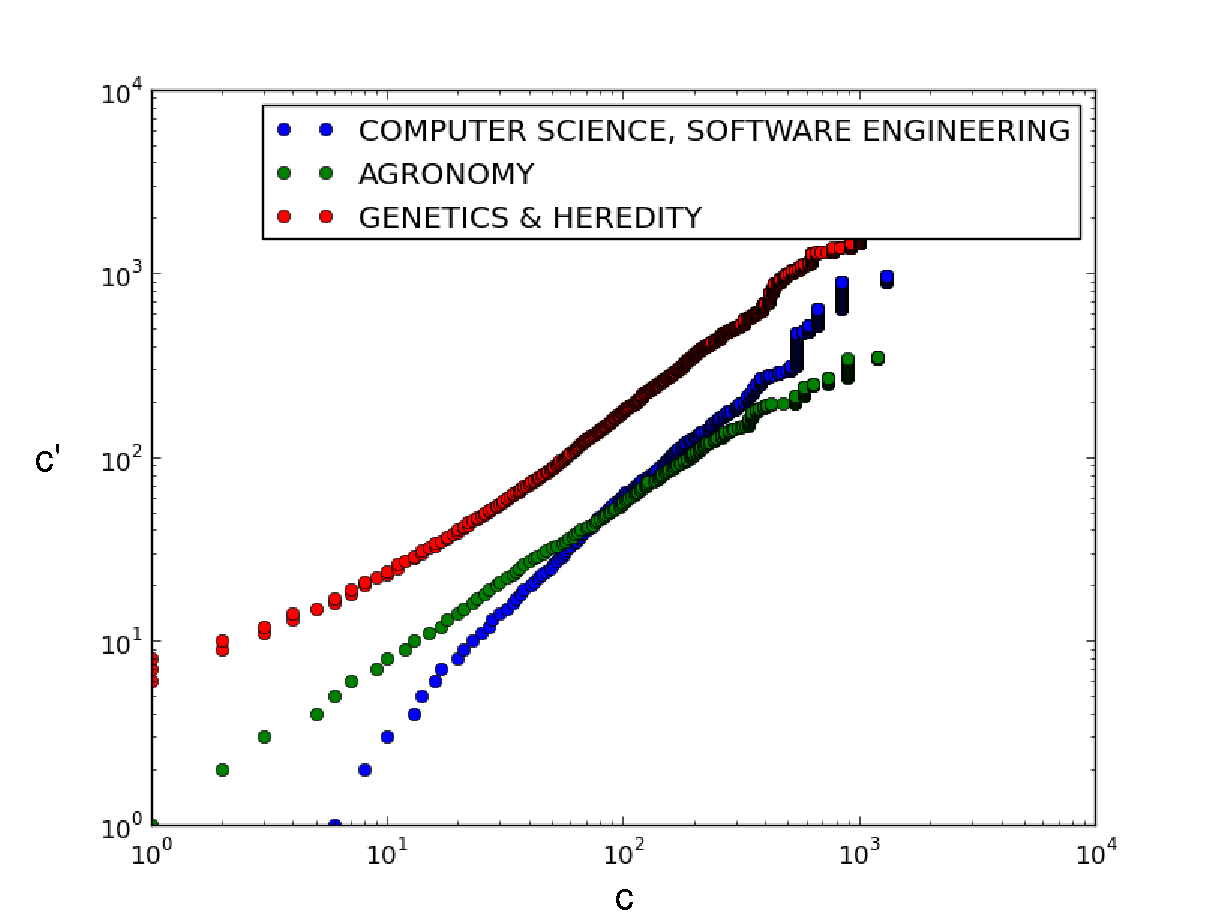
\includegraphics[width=.8\textwidth]{radicchi.pdf}%
\caption{$c'$ vs $c$ adapted from \cite{10.1371/journal.pone.0033833} and reproduced with our data set. We can see that the scaling follows the relation: $c' = ac^{\alpha}$ where
a is a pre-factor and $\alpha$ is a field dependent scaling factor.}
\label{fig:radicchi_citations}
\end{figure}

\pagebreak
\newpage


\section{Biases in citations}

In 2005 Hajra et al. were \cite{Hajra200544} were among the first ones to suggest a temporal aspect in citation dynamics and decided to look at the impact that age has on citations. By looking at the citation dynamic of a 
set of papers, they found a critical time $t_{c}$ of 10 years, after which the rate at which citations are gathered drop significantly, indicating that papers have approximately a \textit{lifespan} of 10 years. In another paper in the 
following year \cite{Hajra2006575}, the authors suggest that the \textit{rich get richer} mechanism might require to be connected with an aging of the publications in order to take into account the obsolesce
of scientific publications. In Publication II we confirmed this property, showing that the typical life cycle of a paper is becoming shorter in time. Fig.\ref{fig:peak_decay} shows the evolution of the time to reach the 
peak of citations for top papers in a selected number of fields.
\begin{figure}[htpb!]
\centering \large
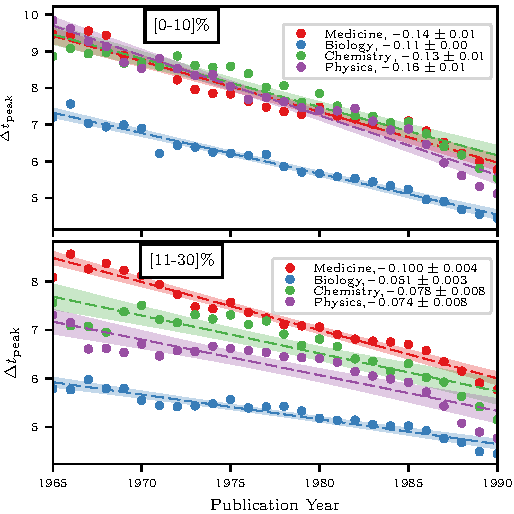
\includegraphics[width=.8\linewidth]{Figures/Fields_Peak_stats_Mean.pdf}
\caption{ Time evolution of the mean values of time to peak $\Delta t_{{peak}}$ for top 10$\%$ (top) and [11-30]$\%$ percentiles (bottom) of our ISI dataset. $\Delta t_{\mathrm{peak}}$ 
represents the time elapsed between the publication of a paper and the year in which it reached its maximum yearly citation count.
The mean value $\langle \Delta t_{\mathrm{peak}} \rangle$ decreases linearly in time. The linear fit, $95\%$ confidence interval and the slopes of the linear fits are also shown. Figure adapted from Publication II.}

\label{fig:peak_decay}
\end{figure}

While the average suggests that papers are being forgotten within a limited period of time, other works have been looking at the opposite phenomenon, the one of \textit{sleeping beauties}, i.e.
scientific papers that remained almost citationless for a long period of time only to become suddenly highly influential and cited \cite{Ke16062015}. The authors designed a Beauty coefficient defined as
$B = \sum_{t = 0}^{t_{m}} \frac{\frac{c_{t_{m}}- c_{0}}{t_{m}} * t + c_{0} - c_{t}}{max \{1,c_{t}\}}$ , where $ c_{t_{m}}$ is the maximum number of yearly citations gathered at time $t_{m} \in [0, T]$ and $T$ is the time 
at which the coefficient is measured. The coefficient 
therefore quantifies how "unexpected" the citation history of a paper is, with $B=1$ being the coefficient for a paper that grows linearly at a steady rate. One of the most interesting results of the study is that
sleeping beauties, albeit appearing to be extreme cases, are impossible to distinguish from the core of all papers, as there is no minimum $B^{*}$ value that allows to define a sleeping beauty as such. While most 
values of $B$ are shown to be low, the authors conclude that it is an intrinsic property of scientific output to have a vast heterogeneity in the times at which recognition takes place. These results
make particular sense for field such as Physics or Chemistry, where the theoretical and experimental sides of the same field are not always synchronized. 

One of the most evident examples of this asynchronism is the recent experimental discovery of the Higgs
boson, the existence of which was originally proposed in the 60s \cite{PhysRevLett.13.508} but was confirmed only in 2012 thanks to the development of the LHC at CERN in Geneva \cite{Aad20121}. The search of the boson was lagging so much behind that still 10 years after the 
theoretical breakthrough the hopes of a search for the Boson seemed remote despite phenomenological studies regarding its discovery had already started \cite{1201.6045}, as one of these studies points out \cite{ELLIS1976292} :

\textit{“We should perhaps finish our paper with an apology and a caution.
We apologize to experimentalists for having no idea what is the mass of the Higgs
boson, ..., and for not being sure of its couplings to other particles, except that they are
probably all very small. For these reasons, we do not want to encourage big experimental
searches for the Higgs boson, but we do feel that people doing experiments vulnerable to the
Higgs boson should know how it may turn up.”} 

The temporal aspect of recognition of older theoretical breakthroughs was a central source of inspiration for Publication I. In the paper we looked at the time lag between the publication of Nobel discoveries and 
the conferment of the prize, finding that it has been increasing at a very high rate, to the point where the original authors might pass away before seeing their discoveries empirically confirmed as shown
in Fig.\ref{fig:nobel_delay}. These findings
led us to conjecture that we are potentially in presence of two opposite scenarios: either the frequency of groundbreaking discoveries is
decreasing or, conversely, it could be that too many significant results are being published and that older discoveries are being awarded in order not to forget worthy winners.

 \begin{figure}[h]
\centering
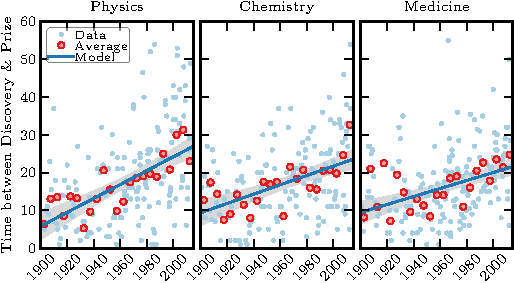
\includegraphics[width=.8\textwidth]{combined_PrizeSinceDiscovery.pdf}%
\caption{Time lag between discovery and Nobel prize vs year in which the prize was awarded for Physics, Chemistry and Medicine, created with data from Publication I. For each Nobel prize we searched bibliographic material on the author in order to
identify one or more publications that could be directly associated to the awarding of the Nobel prize. The blue dots represent individual discoveries, while the red dots
are a 5 year average over all awards in the bin. We can see a clear increase in average lag as well as the presence in more recent year of extremely high values (lag $\approx 50$ years). Figure adapted from Publication I.}
\label{fig:nobel_delay}
\end{figure}


Furthermore, one author might not be even aware of certain scientific works if he has not had the chance to read them or to search them
efficiently. Even though the limitations of access to scientific knowledge might have become less relevant in modern times thanks to the rise of the Internet era and immediate access to online catalogues, at the same time the possibility
to browse more recent material has consequently introduced a change in the way authors update their knowledge. The effects on the scientific community were rapid, as in 2003 already De Groote et al. \cite{pmid12883574}
showed through a survey that general users of scientific material prefer digital copies to printed ones. 
The constant need for immediate access to recent scientific knowledge has become such a relevant aspect of science itself that it has led to suggesting a ranking of journals in terms of the speed at which their publications 
complete their cycle \cite{JournalRankingSchemes}. 

An interesting study in the impact of online available material on citation patterns came in 2008 when Evans \cite{Evans395} studied the 
effect of online availability
of journal issues within the citation patterns of the journals and reported that the rise of online available publications shifted the citation patterns. The results showed that the more journals started to appear online, the more the reference list tended to be pointing at more recent discoveries and caused a \textit{concentration}
of citations towards fewer articles and fewer journals, an effect the authors claim is caused by hyperlinking, i.e. the search of further bibliographic material from the reference lists of papers previously read.

Recently however the claim has been challenged by Verstak et al. \cite{DBLP:journals/corr/VerstakASHILS14} as well as by Pan et al. \cite{DBLP:journals/corr/PanPPF16}.
Verstak et al. used Google Scholar Data to analyze all publications available between 1990 and 2013. The authors calculated the fraction of references in these papers pointing at least 10 years before the year of publication
for each paper and found that such fraction is actually \textit{increasing} in time. Furthermore, they noticed that the value of the change over the second half of the period 
studied was much larger than in the first,
with the former matching the period in which digitalization has took place (2001-2013). The authors therefore concluded that the accessibility of older material has allowed scientists to cite the most suited paper that they were
able to find, regardless of the time at which it was published. The latter paper by Pan et al. instead devised a model to test Evans' hypothesis which builds a citation network in which papers choose whom to cite 
both by "browsing" (i.e. by searching previous publications freely) and by a \textit{redirection} link-formation mechanism in which knowledge is found
by following the reference list of a source article previously browsed. By controlling the rate at which these two processes take place the authors
simulated a spark in the redirection mechanism, representing the availability of online journals. The model showed that the redirection mechanism had very little impact on the average age of citations, while the growth of the system
appeared to have a much more significant role. 

The constant increase in scientific works might limit the ability to physically and mentally keep track of all relevant publications being published. This might be among one of the
greatest limiting factors in citation patterns, as it has been reported 
 \cite{doi:10.1108/00012530910932267} that scientists read more papers, yet
dedicating less time on average to each one. 
The temporal dimension of the 
citation selection process has been the key source of inspiration for Publication II, where we suggest that the increasing number of publications causes a constant shift in focus towards more recent papers, therefore
shortening the citation life cycle of papers both in terms of time to reach their peak in popularity, as well as in terms of time needed to stop gathering significant citations after the peak. Fig. \ref{fig:attention_decay} shows the main results
of the analysis.

\begin{figure}[htpb!]
\centering \large
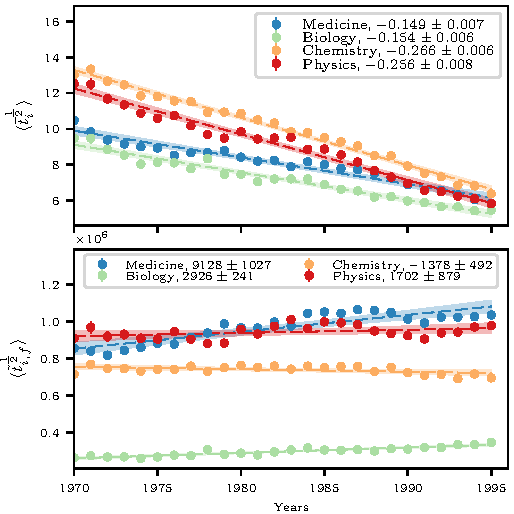
\includegraphics[width=0.8\linewidth]{Figures/LastAbove_0_10_5_finalPaper.pdf}
\caption{ The evolution of the half life of papers after the peak $\langle t_{i}^{\frac{1}{2}} \rangle$ in terms of absolute time (top) and $\langle \widetilde{t}_{i,f}^{\frac{1}{2}} \rangle$  in terms of the number of publications (bottom)
for the four different fields and for the top 10$\%$ percentile. For each paper we calculated the time
required for the publication to drop below half of the number of citations gathered in its peak year. We then proceeded
to average the values for papers published in the same field and peaking in the same year. The half life has been calculated both in terms of number of years and in terms of number
of paper published within the field in the same time interval. 
The linear fit, $95\%$ confidence interval and the slopes of the linear fits are also shown. The dashed line represents the linear fit. Despite its noisy behavior, the
renormalized half-life shows a relatively stable trend throughout the years, possibly with the only exception of Medicine and
Biology, which show a slightly rising pattern for recent time. Figure adapted from Publication II.}
\label{fig:attention_decay}
\end{figure}

Another aspect that influences citation choices is one that looks at the role that the individual authors play. Science is not only a philosophical endeavour, but also a social system where scientists personally interact
and collaborate and therefore are more exposed to works coming from a familiar set of collaborators or, in general, people working in the same area of research. Early research in fact showed that \cite{ASI:ASI10369} intellectual ties based on shared content surpass friendship as a predictor of reciprocal citation. Similarly, Persson et al. \cite{Persson2004} showed in 2004 that collaboration leads to a positive effects in the success of a paper, in particular if
the authors come from different countries.
This can be seen as a success linked to the possibility of the same work to be pushed forward at twice (or more) the same rate as a single author paper in different
"market pools" of customers, i.e. potential citers.  Furthermore, in 2004 Gl{\"a}nzel et al. reported that multi-authorship increases the chances of self citation \cite{Glanzel2004}, with the number of authors not being a factor though. However, the authors point out that
the most dominating contribution of multi authorship is the increase in foreign citations, thus showing the social contribution of a multi author paper in terms of geographical advantage. 

The topic of self-citations is
a highly debated one in a world where citation metrics are used as tools to quantify careers and quality of research. The same author showed in another paper in the same year that  self citations are an \textit{"Essential part
 of scientific communication"} \cite{Wolfgang2004}, but that its contribution plays a higher role in the immediate times after publications. This result, linked with empirical evidence of self-citation being correlated with publishing on average in journals with
relatively low impact shows that this trend might be linked to the need of a "push" in fame, hoping for success to accumulate from there. However, while self-citation does appear to have an impact on citation counts,
it is not clear whether the correlation is linked to a matter of \textit{visibility}, i.e. trying to put forward one's results as a "bandwagon" effect, or rather a matter of \textit{quality}, as one author
mentions its own best works as a basis for future ones \cite{Fowler2007}. More recent results confirm  \cite{10.1371/journal.pone.0033339} that the trend is still significant, yet retaining different patterns in different fields, due to the 
possibility of certain fields to have many groups working on independent topics, thus focusing the selection of cited material from a smaller subset of works. The authors also report that a higher propensity in inter-author-citations
leads to a higher chance of inter-citations of the second order, with collaborators of collaborators being more likely to be cited. 

Authors might also influence their own career retroactively as shown by Mazloumian et al. \cite{10.1371/journal.pone.0018975}. The authors
found that groundbreaking results by an author have a positive impact on their own previous literature, therefore creating a status of authority for the author even though the earlier works
might not be necessarily related to the successful recent ones both in terms of topic and intrinsic scientific quality. The role of prestige in science is so critical that it has been
suggested to also be a bias within the peer review mechanism \cite{ASI:ASI22784}. This psychosociological mechanism that enhances the career of already successful scientists
based on their academic reputation is often called \textit{Matthew Effect} and its impact on science has been discussed since the 60's \cite{MatthewEffect}. In general, a citation bias towards successful papers (preferential
attachment) and one towards successful authors (Matthew Effect) shows that the citation mechanisms are not only based on scientific necessity, but are also based on individual and collective aspects that emerge from the
human interaction between scientists. Finally, it is worth to mention that there are plenty of other factors that influence citations, such as journal-dependent factors, field-dependent factors
and technical ones \cite{doi:10.1108/00220410810844150}, which will not be analyzed for the sake of brevity.






\section{Modeling}

The previous section showed how many factors and biases play a role in the mechanisms underlying the decision of which papers will appear on a reference list, with empirical results showing heterogeneous results within
the same field of analysis. It is therefore not surprising that the pursuit for a mathematical model that could correctly reproduce the properties of citation mechanism has been a challenging one, which scientists however
were eager to undertake in order to shed more lights on the way science itself works, focusing in particular on the temporal aspect of the models.

The earliest and most successful attempts at modeling citation dynamics lie in the \textit{rich get richer} or, technically speaking, \textit{preferential attachment} mentioned in the previous sections . Despite the original idea was already
formulated in de Solla's work \cite{deSollaPrice510}, it was Barab{\'a}si in 1999 who was able to mathematically describe it exhaustively \cite{Barabasi509}.
In his work, Barabasi suggests a model (PAM) in which the probability (or attachment rate)
$A$ of a paper  of receiving another citation from a new paper is directly proportional to the number of citations $c$ citations previously collected: $A (c) \propto c$.
This mechanism is able to explain
the citation distribution both from a qualitative point of view (its fat tailed behaviour) as well as numerically, confirming an expected value extremely close to 3 for $\alpha$. 
Interestingly, the model was applied to a vast amount of complex systems, with particular success in biology \cite{Barabasi2004,Jeong2000}, of which citation dynamics represent one of the examples.

A confirmation of the validity of the preferential attachment mechanism came in 2005 with Redner \cite{RednerStatistics}, who reported that the attachment rate is indeed linear, leading to a double paradox: the linear attachment rate 
shown by the data should lead to a power law distribution for citations, while data shows that the form is log-normal, which in turn would require an attachment rate of the form
$A_{c} = \frac{c}{1 + a \ln(c)}$ with $a > 0$. Despite confirming empirically the validity of a linear form of preferential attachment, Redner suggests that the underlying assumptions
behind the preferential attachment model, when applied to science, might be not completely realistic, as the model implies a full knowledge of all the corpus of existing papers, a
challenge which has its limitations both in terms of accessibility as well as in terms of memory. 


As we saw in the previous section however, it is fundamental to introduce the  question of time dependence within the modeling framework. While theoretical works tried to tackle the topic from a purely mathematical standpoint \cite{Amaral2000,PhysRevE.68.056121}, it 
was Hajra et al. \cite{Hajra200544} in 2004 who applied it with success to the modeling of citations. 
The authors followed the previous theoretical works and formulated a functional form for the attachment rate of 
$\Pi(c,t) = C(c)T(t)$, where $C(c)$ and $T(t)$ are generic functions and where the attachment rate is assumed to be separable. The authors then tried to identify the functional form for the temporal aspect that would best fit the data through the analysis of the distribution of citation ages $Q(t)$, i.e. the raw distribution
of the fraction of citations with age $t$. In order to do so, the authors took
into consideration the stochastic nature of the rate at which new citations appear, i.e. the rate at which new papers are published. Therefore by empirically estimating from their data sets a publication rate
of $n(t) = a(1 - e^{-bt})$ they were able to renormalize the distribution and obtain a functional form of $T(t) = \frac{Q(t)}{n(t)}$. Comparing the model with the collected data, the authors identified
two  distinct regimes of power-law decay of the distribution: $T(t)\sim t^{-\alpha_{1}}$ for  $0<t<tc$  and $T(t) \sim t^{-\alpha_{2}} $ for $t>t_{c}$ where $t_{c} \sim 10$ is the expected lifespan of a paper mentioned earlier.

In Publication II we proposed a model for the process of gathering new citations as a \textit{counting process}. In this ultradiffusive framework, the arrival of a new citation is hypothesized to be  correlated to an earlier event or a combination of events.
Therefore, 
ultradiffusion
proposes that the pattern of events emerges as a consequence of an underlying hierarchy of states, in which a more recent event is more likely to affect the future ones. Our results, that show an exponential fall
in citation after reaching the peak, which is slowly transitioning into a power law pattern is coherent with the hypothesis of an ultradiffusive process driving the attraction of new citations.
This framework is known to be 
able to explain the evolution of the response to new pieces of information online \cite{ghosh_information_2013}, allowing us to draw a comparison between the way in which attention is dedicated to new publications and the way
readers react to news. 


A further improvement on the PAM came in 2008 with a work by Wang et al. \cite{Wang20084692}. Their model proposes to not separate globally the dependence of the attachment rate on the two variables, considering the aging
process to be related not to the whole paper, but to the citations themselves. The logic behind this idea is that a paper that has received a lot of attention lately (a sleeping beauty for example) will be more likely
to gather new citations if compared to a paper published in the same year, with a similar citation count, but having failed to receive citations recently. Therefore, the authors express the rate as $\Pi(c,t)  \propto \sum_{t} c_{i}f(t_{i}) \propto  \sum_{t} c_{i}exp(-\lambda t_{i}) $,
where $k_{i}$ are the citations gathered in year $t_{i}$ and the exponential form for the weights is taken from fitting data, a scheme they call Gradually-vanishing Memory Preferential Attachment Mechanism (GMPAM). 
While the empirical data shows a good accordance the model, the authors admit that the model is somewhat excessively complicated, as it requires to calculate weights for decades of citation data coming from
  different citation pools (field and geographical biases above all) that require to fine tune the value of $\lambda$ case by case. The authors therefore proceed to simplify the model, by observing that the most 
  significant temporal contribution to the attachment rate comes from the most recent number of citations, i.e. the number of citations gathered in the last year. The temporal aspect therefore it's taken to be
  as a \textit{memory effect}, that makes the older citations be "forgotten", giving priority to papers that are riding a popularity wave. The updated model, called Short-term Memory Preferential Attachment Mechanism (SMPAM) thus expresses
  the attachment rate as $\Pi(c,t) \propto c_{t-1}$. 

Similarly, other authors have decided to focus the modeling part only to reproduce certain aspects of the citation dynamics with still a focus on the temporal aspect.
In 2001 Burrel was able to confirm that a stochastic process that assigns citations to publications 
based a non-homogeneous Poisson process \cite{Burrel2001} is bound to produce articles that will remain uncited. In 2009 Wallace et al \cite{Wallace2009296} tried to model the citation distribution of publications by separating the citation curve in different areas, developping in particular a model able to quantify the impact
of uncited papers in the citation distribution. The authors hypothesized that the probability for a certain paper to receive an initial citation depends only on the number of articles $N_{A}$ published in the same year
 and the number of references $N_{R}$ available in the following year, with citations being given randomly through a Poissonian distribution, given the size of the two variables. The authors then limit the 
 probability of citing an uncited paper to the field-dependent rate at which uncited papers are cited for the first time. It therefore follows that the pool of available references is reduced to $\beta_{I}N_{R}$, where $\beta_{I} \in [0,1]$ is extracted
 from the data, and that the probability for a single paper to fail to receive any citations is:
$\Phi_{I} = e^{-\beta_{I} (N_{R}/N_{A}) }$. 

 
In 2009, Newman \cite{0295-5075-86-6-68001} published a study which added to the temporal aging process the aspect of novelty, the so called
\textit{first mover effect}.  The idea behind the work is that science is based on the production of new results and therefore there is an intrinsic advantage in the being the first ones to publish a new result in a field,
since future works are bound to cite the paper introducing the novelty. In his paper, the author works with previous models based on preferential attachment to build a new one where on average newly published papers cite
$m$ earlier papers, chosen proportionally to the number of citations $k$ they already have, plus a variable $r$ needed to ensure
that uncited papers still have a nonzero probability of being cited. From this model one can calculate the average number of citations $\gamma$ a paper is expect to receive at time $t$ as: $\gamma(t) = r(t^{-1/(\alpha - 1)} -1)$, where $\alpha =  2 + r/m$.
Therefore, it follows that older papers (i.e. $t \rightarrow 0$) should on average receive far more citations than
those published later, even taking into consideration the the fact that later
papers have less time to gain citations.

These results are somewhat in contrast with the previous discussion regarding obsolescence and the time span of papers. 
However, Newman himself points out that the first mover advantage is limited to scenarios in which the results
are not part of a  larger, already established field, but rather represent the emergence of new subfields or fields altogether, as their analysis of citation data in fact seems to confirm. 


In 2011 Eom and Fortunato  \cite{10.1371/journal.pone.0024926} published a paper in which the aspect of the \textit{burstiness} in science is tackled. Burstiness is a sudden and intermittent modification of the 
frequency of an event,  which has been known to play a fundamental role in many human dynamics \cite{0295-5075-81-4-48002,PhysRevE.83.025102}. In this context, burstiness represents all sorts of inhomogeneous fluctuations that
lead to a sudden and unexpected rise in the citation count of a paper, which can be expressed as $ \Delta c/c = [c(t+\delta t)^{i}_{in} - c(t)^{i}_{in}]/c(t)^{i}_{in}] $, where $c(t)^{i}_{in}$ is the number of incoming citations
a paper received at time $t$ measured in years. This rate therefore measures the relative change in citations during the period of time $\delta t$, compared to the history of citations of the paper. Data shows that the distribution
of these rates is fat tailed for $\delta t = 1$, showing therefore that it is possible for a paper to suddenly receive orders of magnitude of citations more than they ever did, especially during its early years. Similarly to what happens to sleeping beauties, burstiness shows that there can be stochastic driving forces that cannot be ignored and that a linear model with no memory
or time dependence cannot grasp. The authors therefore propose a model still based on the preferential attachment model, where however each papers has an intrinsic \textit{attractiveness} that depends on time. The result is a model in which a new paper $i$
cites $m$ new papers, with the probability of a certain paper $j$ to be cited described as : $\Pi(i \rightarrow j ,t) \propto [ c^{j} + A_{j}(t)] $. For the form
of the attractiveness the authors assume an exponential decay $A(t) = A_{0} exp^{-(t-t_{0})/\tau}$, where $\tau$ is the time scale at which the temporal dimension plays a role, with initial attractiveness taken from a power law in order 
to best fit the data. Once again, we have a model
where a linear preferential attachment is mixed with a temporal dimension, which in this case takes into account random fluctuations of the citation history of the paper that
alter the expected individual citation trajectories. Attractiveness can be seen as proxy of an intrinsic \textit{quality} of the paper, which is explicitly separated by the success of a paper in terms
of citation. The model therefore suggests that citations do not represent the absolute measure of the quality of the paper, but that rather they are a probable (but not guaranteed) consequence
of papers of high quality (attractiveness). However, with citations and preferential attachment still being a fundamental driving force of the citation market, an initial failure to gather an initial minimum number
of citations might be sufficient to prevent a high quality paper from rising to notoriety. 

In 2015 Wang et al. \cite{Wang127}, including the original proponent of the Preferential Attachment Model
Barab{\'a}si tried to further expand the concept of separating the driving force of citation and the one of fitness of the individual paper, by proposing an attachment rate of the form:
$\Phi_{i}(t) \propto \eta_{i}P_{i}(t,\mu_{i},\sigma_{i})c_{i} $, where $\eta$ is the fitness of the individual paper and $P_{i}(t,\mu_{i},\sigma_{i})$ represents the aging process of the ideas introduced by the paper. The separation of fitness
from aging (i.e. it's not the fitness that decays, but rather the \textit{novelty}) comes at a cost, as the authors needed to introduce two new parameters, represented by the immediacy $\eta$ of a paper and
its longevity $\sigma$ which determine the time at which a paper reaches its peak of notoriety and how long its notoriety will last respectively. The model is therefore able
to predict the future citation trajectory of a paper, given a previous window of time during which its intrinsic parameters can somehow reveal themselves and be quantified
through a least square fit method. Furthermore, the authors managed to quantify the importance of the individual contributions within the attachment rate formula, finding that
the dependence on the number of citations (i.e. the classical model) is triggered only when a paper crosses the threshold of seven citations, below which it's the paper attractiveness that 
dominates.



\chapter{Network Structure of Science} \label{Network Structure of Science}

De Solla's seminal paper \cite{deSollaPrice510} begins like this: \textit{"This article is an attempt to describe in the broadest outline the nature of the total world network of scientific papers. We shall try to picture the network which
is obtained by linking each published paper to other papers directly associated with it."}. Already at the beginning of the study of scientometrics it appeared evident that
science needed to be tackled from a global perspective, analyzing the connections that link scientific papers to one another.
 Similarly, two co-authors of the same paper
can be linked together, as well as two scientists who have collaborated with the same scientist as the famous Erd\H{o}s number grasps \cite{10.2307/2317868} 
\footnote{The Erd\H{o}s number measures the distance in terms of collaborative steps between the Hungarian mathematician Erd\H{o}s and his direct or indirect collaborators. Anyone
who has collaborated with him has a Erd\H{o}s number equal to 1. All their collaborators have a EN of 2 and so on.}. In general, the 
intrinsic collaborative nature of science either by cumulative contribution (the shoulders of giants) or by direct collaboration has led to the creation of a massive
scientific network that can be analyzed in many of its levels, where both its nodes and links can take many forms, with nodes representing papers as well as authors, institutions or countries and links representing
citations, co-authorship, shared funding etc. 

Graph theory showed for the first time the potential of network research for practical problems in the famous work by Euler in 1796; by simplifying the bridge and road structure of the
city of K{\"o}nigsberg in terms of nodes (land masses) and links (bridges), the Swiss mathematician was able to negatively answer the question: is it possible to perform a path around the city that
crosses each bridge of the city exactly once? For a long time graph (or network) theory remained confined mainly as a branch of topology in theoretical mathematics \cite{Cayley1881} until the middle
of the 19th century when the earliest structured books appeared  \cite{0817633898,9782746232150}, allowing the developments in the theory to spread
to new fields \cite{0123242509}, including sociology, where researchers understood that a matrix based representation, i.e. one of the underlying bedrocks of network theory,
of social ties could be beneficial for the study of social structures \cite{Luce1949,10.2307/2088670}. The breakthrough came in 1959 with Erd\H{o}s and R\'{e}nyi's work on
random graphs \cite{citeulike:4012374} in which the authors studied
the invariant properties of graphs generated through a stochastic model that distributes a fixed number of links across all possible node pairs. The ER model turned out to have strong
analogies with statistical mechanics \cite{COHEN1988113} and was later used as a fundamental tool for studies that required a network based structure, in particular 
for models in epidemiology \cite{pmid7608641,Keeling859}. 

In general, the ER model allowed the rise of what are called \textit{generative models}. 
These models aim at reproducing the statistical properties of the observed networks \cite{1608.00607}, yet keeping the most important features (usually
the degree distribution or the average degree) of the network
statistically constant, while allowing for the edges to be distributed at random. Generative models therefore act as tools for generating null-hypothesis that can be tested statistically,
allowing to identify which properties in real networks are statistically relevant, with applications to multiple fields \cite{Connor1979,Gail1977}. Among the attempts, de Solla Price
contributed with the earliest definition of the rich get richer mechanism \cite{Price1976} that would later be made popular by Barab{\'a}si and Albert, who
showed its potential \cite{Barabasi509} as a tool to describe the emergence of scale-free networks. Barab{\'a}si and Albert's paper was part of a period
of extreme interest for network theory studies as the rapid accumulation of data of large networks thanks to the digitalization of society, allowed
for the first time to provide a robust set of data that could be used to test previous models. While the ER model had been extremely successful due to 
its simplicity, the evidence of different properties in real networks required the development of new models, which rapidly took place \cite{Watts1998,Albert2002}


Since then, network theory has been applied in a large spectrum of fields, dealing with non-trivial network structures that required methods and algorithms tailored to specific types of network problems, leading to a whole new field, often referred to as \textit{complex networks}, in order to differentiate it from Graph Theory. As the theory developed,
the application of its methods to publication data became a fertile branch of the field. 
This Chapter will first go through the basics of network theory, in order to provide a mathematical foundation for the rest of the chapter, in which the most significant
applications to scientific networks will be discussed.

\section{Networks}
A network, also called graph, is a collection of nodes connected by links. Mathematically it is represented
by $G = (V, E)$ where $V$ is a set of $N$ nodes and $E$ is a set of $M$ links (or edges) connecting pairs of nodes. 
A convenient way to represent a network is through its \textit{adjacency matrix} $A$, which fully describes the graph.  Its
elements $a_{ij}$ are 1 if there is a link connecting node i and node j and 0 otherwise. If
$A$ is symmetric the graph is undirected as all of its links go in both directions. It is often assumed that there are no self loops, i.e. $a_{ii}=0$
for all i. In this simplest scenario, the elements of the matrix are usually binary and symmetric, thus only indicating whether two nodes have a connection or not.
However, more sophisticated networks can be built by modifying these conditions:
\textit{Directed graphs} take into account the directionality of the links by dropping the symmetry requirement, while \textit{weighted} graphs drop the binary requirement
for the elements of the matrix, thus quantifying the "strength" of the link. An example are mobile call networks, in which $a_{ij}$ can indicate the number
of calls between user $i$ and $j$, or the total time spent between two users \cite{Onnela01052007}. Networks in which most elements of the adjacency matrix
are 0s are usually called \textit{sparse}, while in the opposite case they are called \textit{dense}. Sparse matrices, which
are not rare at all \cite{Davis:2011:UFS:2049662.2049663}, can represent a problem computationally
in terms of storage space since, if stored in matrix form, $N^{2}$ entries need to be stored, most of which do not carry information.
Fortunately, the disadvantage can be turned in an advantage by using \textit{adjacency lists} in which each row $i$ enumerates
the neighbors of the node along with the value of the edge in case it is required. 
Recently, there has been a need to analyze many different kinds of network structures. For example, temporal networks take into consideration the intermittent activity of the edges in the network, thus adding 
a temporal dimension to the analysis of complex networks \cite{Holme201297}. Multilayer networks instead deal with
systems in which nodes exist in one or more of multiple layers and where links can connect nodes also across layers \cite{Kivela2014,Boccaletti2014}.
Such networks can be useful to analyze interactions in social systems, where each layer represents a different kind of interaction and where
not all users are equally active in each layer, or might not be active at all in some of them \cite{Szell03082010}.




\subsection{Degree}
The degree $k_{i}$ of a node is the number of nodes that node i is connected to. 
It can be derived using the adjacency matrix $A$ as  $k_{i} = \sum_{j} a_{ij} $, i.e. the sum of the nonzero elements of
row $i$. In case of a directed network two separate degrees are considered : $k^{in}_{i}$ and $k_{i}^{out}$, which differentiate
between the degree calculated respectively over the columns or the rows. The average degree  $\bar{k}$  of a network is the average value of individual degrees 
  $\bar{k} = \frac{\sum_{i} k_{i}}{N} $, where $N$ is the number of nodes in the network. Again, it is possible to define an average $\bar{k}^{in}_{i}$ and $\bar{k}_{i}^{out}$ for directed networks.
  
When analyzing a large network, it can be useful to look at the overall distribution of the degree values for the nodes of the network, as with an increasing number of nodes it 
becomes necessary to analyze them statistically. In the ER model \footnote{This formulation was presented in the same year by Gilbert \cite{gilbert1959} and is statistically equivalent
to the ER model.} each link exists with probability $\frac{M}{\binom{N}{2}}$, leading to the probability of node $i$ to have degree $k$ to be the 
probability of having $k$ times successful
Bernoulli trials, thus converging to a Poissonian distributions as the size of the network grows, with $\bar{k}$ remaining constant.
However, empirical evidence \cite{Barabasi2004degree}
has shown that real world networks have a dramatically different behaviour when it comes to degree distribution.

While the ER model predicts a large amount of nodes sharing
similar degree values, social, biological and transportation network among others, revealed themselves to have fat-tailed distributions \cite{Clauset2009}, i.e. they showed the existence of nodes with large degree called \textit{hubs}, along with a 
vast amount of nodes with low degree values. In 1999, Barab{\'a}si and Albert proposed a different model, in which the network is generated by adding new nodes and
connecting
them proportionally to the degree of the previously existing nodes, through the Preferential Attachment Method already introduced in the previous chapter. In Fig.\ref{fig:degree} we can see a comparison
between the appearance and the degree distribution of a random networks compared to a scale-free network. 
 \begin{figure}[h]
\centering
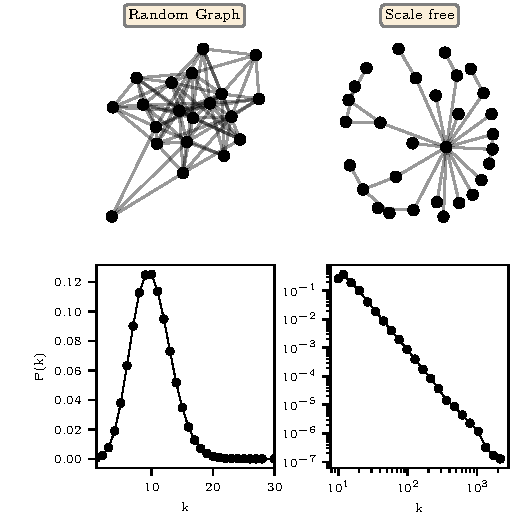
\includegraphics[width=.8\textwidth]{degree_histogram.pdf}%
\caption{Difference in topology and degree distribution between a random graph (left) and a scale-free network (right). The random network has its degree distribution heavily
centered around its average, with no significant outliers. In the scale-free model instead, degrees can span multiple orders of magnitude.}
\label{fig:degree}
\end{figure}
   
Another fundamental property of degree  is linked to the concepts of \textit{assortativity} and \textit{resilience}. Assortativity is used to investigate what is the tendency in a network for nodes with similar 
degree to be connected \cite{PhysRevLett.89.208701,Newman2003} and is therefore often expressed as degree-degree correlation. In a network with high assortativity, high-degree nodes are likely to be connected
and tend to avoid connections to low-degree nodes. Similarly, a network is disassortative if high degree nodes tend to avoid being linked to each other and prefer being connected to lower
degree nodes. In both the ER and Preferential Attachment models, there is no correlation between degrees; in the ER model
links are given randomly, thus an absence of correlation is to be expected for large graphs, while in the PA model the evidence is less trivial, but it comes from the fact that hubs have a tendency to get links
from all new nodes, thus failing to select connections to specific nodes. Interestingly, real life networks show different scenario, with certain networks being assortative (power grids, social networks) and other disassortative (WWW, protein-interaction
networks), thus requiring more sophisticated models to be able to reproduce these features \cite{Callaway2001}. A direct consequence of assortativity is resilience, i.e. the ability of a network to resist
the attack or failure of random nodes. In a air transportation network for example, this corresponds at how the passenger traffic is affected by the closure of randomly selected airports. Numerical simulations \cite{PhysRevLett.89.208701}
show that a high assortativity is linked to a better chance to resist attacks due to the fact that hubs, which are often fundamental as they allow to distribute "services" to the periphery of the network, are likely to be connected
to each other, thus creating dense cores of highly connected nodes that keep the structure of the network efficient. In disassortative networks instead, hubs are fundamental local service providers and, if shut down,
are more likely to cause an interruption in services. Unfortunately, many communication networks are disassortative \cite{doi:10.1093/comnet/cnv005} and have therefore been often
subject of systematic failures \cite{Sterbenz20101245} due to their structural inefficiency.


\subsection{Clustering, paths and distances}
The clustering coefficient measures how likely two nodes within the neighbourhood of a node are also
 be connected \cite{Watts1998}. Let's consider a node with $k$ neighbours. Among these neighbours there are $\frac{k(k-1)}{2}$ possible links, i.e. the number of ways 2 nodes can be selected if there are k nodes,
 out of which only $E_{i}$ are present in the network. The CC is defined as the ration between the two terms:
\begin{equation}
 C_{i} = \frac{E_{i}}{\frac{k_{i}(k_{i} -1)}{2}}
\end{equation}
In case of weighted and directed graphs the concept can be generalized 
in multiple ways \cite{Fagiolo2007}. The average clustering coefficient of a network is the average $C = \sum_{i} C_{i}/ N$ of the individual clustering coefficients.
 The global clustering coefficient is a similar measure as the average clustering coefficient which looks 
at the clustering of a network from a geometric point of view. It is defined as the fraction of triplets (i.e. a set of 3 connected nodes) that actually form a triangle and can be applied to both undirected and directed networks \cite{Newman2003Complex}.
In an undirected network the average path length between two nodes is defined as $l = \frac{1}{\frac{n(n+1)}{2}} \sum_{i\geq j} d_{ij}$,
where $d_{ij}$ is the length of the shortest path between two nodes. In case the graph is not connected (i.e. there are parts of the networks that are separated), the value of the average path length diverges and is therefore
convenient to compute it individually for each subgraph of the network. The diameter, $D$, of a network is defined as the maximum shortest path between any two nodes in the network. Its name recalls the topologic
properties of circles as it represents the approximate linear size of the network.  

In 1998 Watts and Strogatz published a paper that showed how the currently available models based either on regular lattices or on random graphs were unable to grasp the properties of real networks in terms of clustering coefficient
and path length\cite{Watts1998}. While their analysis of diverse networks (power grids, biological networks, film actors) showed large CC and short paths, the ER model  \cite{Albert2002} is bound to generate networks
with average path length $\propto log(N)$ and have an extremely low value for the CC. They called their networks \textit{small-world networks} in reference to the famous social experiment of the six degrees
of separation \cite{sixdeg}, which was the first attempt at calculating path lengths in social networks. They proposed a stylized model based on a regular lattice, thus guaranteeing high clustering, with a random rewiring
of each link controlled by a parameter $p$. The value of $p$ therefore allows the transition from a regular lattice ($p=0$) to a random network $p=1$. As $p$ increases from 0, local clustering remains high while
paths between distant nodes cause a significant reduction of the average path lengths. With this simple model Watts and Strogatz managed to show how even a small number of short cuts
can transform a sparse, locally clustered network in a small-world one.


\subsection{Communities and modularity}
Between 1970 and 1972 Wayne W. Zachary collected data about the interaction between 34 members of a karate club, during which two instructors had an argument, leading to a split of the group into two, with half of the group
remaining in the club with one instructor and the other half leaving it  \cite{10.2307/3629752}. Based on the difference between the interaction patterns, Zachary was able to devise an algorithm able to automatically
detect in which half a node would lie. This became the first example, and later the benchmark, of a \textit{community detection} algorithm \cite{Fortunato201075}. The idea behind community detection is that networks can be organized in locally highly connected clusters separated one from the other, known as communities. Real world examples are abundant:
metabolic networks are organized into small, highly connected modules \cite{Ravasz2002}, urban areas and societies can be structured in large groups divided by language \cite{1742-5468-2008-10-P10008},  and also network scientists are organized in communities \cite{physics/0605087}. While
communities are easy to qualitatively define, their mathematical definition has been the source of debates as, like in the Karate Network splitting in two roughly equivalent groups, one needs to possess previous information
in order to know how many communities are to be found and what their typical size is.
    
 \begin{figure}[h]
\centering
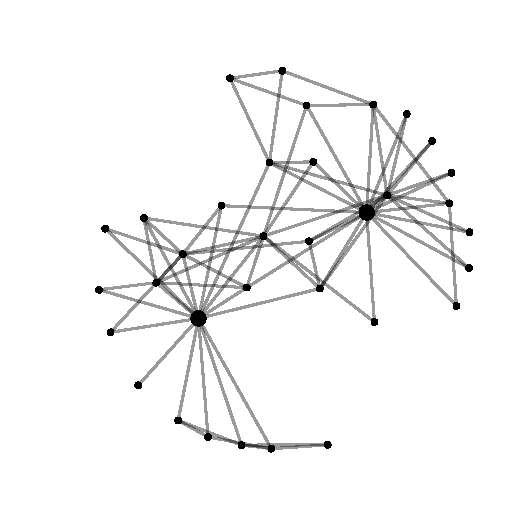
\includegraphics[width=.8\textwidth]{karate.pdf}%
\caption{Visualization of the karate network based on the data from \cite{10.2307/3629752}. The network is visibly structured around the two hubs 
(larger nodes), with clustered communities around each hub and a few nodes acting as intermediaries between the two communities.}
\label{fig:karate}
\end{figure}

As new algorithms attempted to find the most optimal division of the network in communities, it 
became therefore necessary to develop a method able to grasp the quality of the partition of the network. Among the various methods, the most popular one is the one of \textit{modularity optimization} \cite{Fortunato201075}.
This method, introduced by Girvan and Newman in 2002 \cite{Girvan11062002} is based on the idea that a good partitioning maximizes the amount of edges within a community and minimizes the amount of links towards the outside of the community. 
Modularity is therefore calculated as the difference in number of edges within a cluster and the expected number of edges that one would found in a similar network in which
individual nodes retain their degree, but the edges are randomly rewired. In Publication III a similar idea was used to investigate how dense the subgraph of Ego Networks, the graph formed by the neighbours of a specific individual (the ego) and by their mutual relationships, is. 
The EN is the realistic, local perspective of a given node representing the information that it might use in basic decision processes.
We calculated for new nodes joining the EN the fraction of references that stay within the EN, thus quantifying how modular the EN is and
how its modularity evolves in time. We showed that the EN has a sharp initial growth in modularity that saturates within 10 years,
before gradually decreasing as shown in Fig.\ref{fig:ego_modularity}.

Unfortunately, despite its simplicity, modularity also offers some limitations. Fortunato et al. showed in 2007 that modularity optimization is bound to have a resolution limit, i.e. a minimum size
of communities under which the method fails to detect communities \cite{Fortunato02012007}, which can represent an issue as real networks can be organized 
in hierarchical or tree-like structures  \cite{10.1371/journal.pone.0011976}. Furthermore, such resolution limit depends on the size of the network; as a network increases in size
the null model might expect two clusters to have a very low probability to be connected, therefore allowing one single connection between them to be seen as a strong
statistical indicator of modularity, thus merging the two clusters.
Even by trying to introduce a resolution parameter in order to find clusters of various sizes, problems such as merging of subgraphs and splitting
of graphs arise \cite{PhysRevE.84.066122}. Furthermore, another key limitation is the presence of multiple suboptimal solutions \cite{PhysRevE.81.046106} that still offer good results. While other methods are being introduced
with good results, they all come at a cost somewhere, due to the intrinsic loose definition of a community, thus forcing the scientists to perform a trial and error analysis based on the cumulative 
information gathered in the process \cite{Fortunato20161}. To summarize, there is no "Free Lunch" in community detection \cite{Peel2017}.
    
 \begin{figure}[h]
\centering
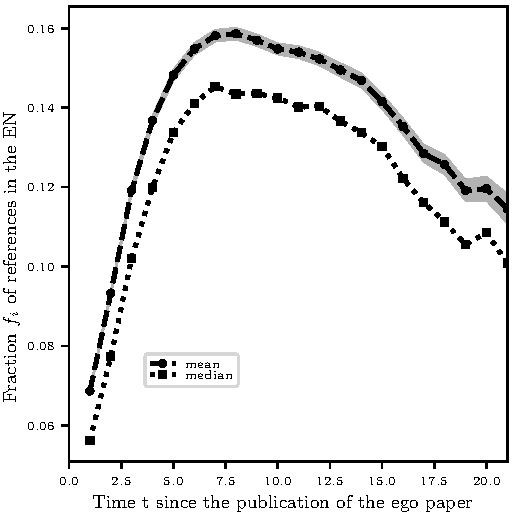
\includegraphics[width=.8\textwidth]{ego_modularity.pdf}%
\caption{Time evolution of the mean and median of the fraction $f_{i}$ of references of papers of the full Ego Network belonging to the Ego Network
as a function of the number of years since publication. In this framework, $f_{i}$ is the EN equivalent of the modularity of the community that is formed around the original paper. 
In the first years $f_{i}$ increases significantly, peaking after $ \approx 7$ years, after which a constant decrease takes place. Interestingly
however, the EN is also getting bigger in size, thus potentially allowing for more references to be part of the EN. Figure adapted from Publication III.}
\label{fig:ego_modularity}
\end{figure}

\section{Author networks}
As we have seen, network theory provides a solid framework with which to investigate social structures. It followed therefore that scientists could use the very same methods to investigate the social structure
of science itself. The main candidate for such analysis are author based networks, i.e. networks in which nodes are represented by individual scientists that are connected according to similarity in their publications.

The most straight forward approach is the one to considers co-authorship networks, in which links are assigned between scientists who collaborate in the writing of a single paper. The first study in the field was performed by Newman in 2001, by studying a dataset of over 2 milion papers and 1 milion authors in Physics, Computer Science and Biomedical research \cite{Newman16012001}.
This work allowed for the first time to quantify the collaborative structure of science with the newly formulated tools of network science. The data showed that the degree distribution, i.e. the number of collaborators
for a single author, follows a power-law behaviour with an exponential cutoff, a result coherent with a power-law degree distribution, with the cutoff being due to a size restraint in the system. The author also reports
that the network of scientific collaborations shows a small-world structure, with authors being no more than five or six steps apart from each other. The network showed also an interesting tendency for authors to cluster,
even though this might be biased by the presence of papers written by 3 or more authors, which, by the network construction rules, create triangles in the network. Newman's work showed the intrinsic social nature of science as a network
of collaborating nodes, with a structure that is coherent with a PAM in which authors with most collaborations are more likely to collaborate with new scientists. However, from
a theoretical point of view, it fails to find an explanation for the coexistence of a  power-law degree distribution and the intrinsic community-based structure, a feature absent in the PAM. 

The matter was further analyzed by Barab{\'a}si et al. \cite{Barabasi2002590}, who confirmed the clustering nature of co-authorship networks with a caveat: clustering, as well as other
 key properties of the network, are time dependent, therefore providing only partial information about the true structure of the network. This work, while reinforcing a preferential-attachment approach to the evolution
 of co-authorship networks, once again introduces the matter of time in the exploration of properties of the scientific community. 
 
 It has been suggested that a major role in the temporal aspect of co-authorship networks 
 may reside in the evolution of the individual careers of the different authors \cite{Wagner20051608}. Sociological considerations \cite{Gursey} can support the hypothesis that the preferential attachment method, that is the 
 phenomenon by which authors with many collaborations are more likely to have new ones,
 is the the driving force only of collaboration only for scientists in the middle of the career (thus also in the middle
of the distribution). The tails of the distribution instead are dominated by either established scientists, who don't require to build up their network anymore, or newcomers who instead fail to act as attractors
 in the network. It therefore follows that one cannot investigate the social structure of science in snapshots, but rather needs to follow its temporal evolution as  \textit{"networks
change over time, both because people enter and
leave the professions they represent and because practices
of scientific collaboration and publishing change"} \cite{Newman2004Connected}. 

Furthermore, one needs to step at a deeper structural level:
 while co-authorships provide the basic framework, it is important to differentiate between the various substructures that exist within a network as evidence shows that the local structure of the network
 has an impact on the citation and co-authorship patterns \cite{10.1371/journal.pone.0057546}. In fact, co-authorship practices are extremely heterogeneous across fields, as in certain applied sciences it is not rare
 to find papers co-authored by tens of authors, thus putting into question the ability of this approach to reflect the social structure of science. In fact, networks of different size need different collaborative behaviours for the 
 their community structure to persist in time. While smaller collaborative groups tend to be based on a core of strong relationships that are self-sufficient, larger groups need a more dynamic structure that
 reaches out to new members in order to survive, similarly to what happens in mobile communication networks \cite{Palla2007}. 

 Even though the co-authorship network is purely abstract in its formulation, it is possible to merge it with physical data, e.g. the location of the institution in which the authors work, allowing to add a 
 geographic dimension to the analysis. Relocation is common in academia, even though scientists usually are not likely to cover long distances, and can play a crucial role in one's career \cite{Deville2014}.
 Similarly, the choices of collaborators are also affected by geographical considerations that can be linked to policy making from individual countries or unions \cite{Hoekman2010662,Leydesdorff2008317}.


 
 \subsection{Ties and careers}
 In a framework in which the career and the connections of individuals change structurally over time, it becomes therefore fundamental to investigate the different nature of the links that connect different authors at different stages of their careers; after all science is not only
 driven by purely intellectual but also by more practical driving forces, such as economical and political matters that can also alter the paths of individual careers \cite{Kaplan2010,Petersen2012}, thus affecting
 the structure of collaborations both locally and in time. Similarly, as the network structures are known to influence team-performance \cite{Guimera2005,PentlandTeam}, it is natural to conjecture that these kinds of mechanisms are 
 reflected in the data of scientific collaborations. 
 
 In order to better understand such effects it is beneficial to investigate the role of the \textit{strength} of the ties between authors as a measure to identify which
 connections are more productive and represent a stronger tie within the sphere of scientific collaboration. This can be done by building a weighted network, where the weight of each link is defined as $w_{ij} =  \sum_{p} \frac{1}{n_{p} -1 }$
 where $p$ is the set of papers where authors $i$ and $j$ collaborate and  $ n_{p}$  is the number of co-authors of paper $p$.  
 Contrary to previous results in social networks \cite{Onnela01052007}, 
 collaborative networks show a unique characteristic: weak ties form the core structure of 
 dense neighbourhoods, with strong ties connecting different neighourhoods. This effect is considered
 to reflect the hierarchical and temporal dimension of scientific careers: as senior researches build strong ties with each
 other over time, they form research groups composed of young researchers \cite{Pan2012Ties,Ke2014}. Even though it is only
 a few strong links between senior scientists that keeps the scientific network of authors together, simulations show that 
 they are fundamental for the efficient spreading of information through the network. 
 
 In an academic world where
 most junior scientists drop out \cite{Pan2012Ties}, which is hierarchically and sometimes unequally structured in its hiring
 system \cite{Clausete1400005} and in which early developments can lead to a cumulative advantage in a career  \cite{MatthewEffect,Petersen04012011}
  it appears evident that the evolution of the social and collaborative structure of scientific interaction is closely related to 
 the evolution of the individual careers of the prominent scientists: their moving forward in the 
 hierarchy of science, projects their connections to a more important role within the scientific network and eventually allows them
 to influence the local properties of the network as they build their own team. 
 
 In 2015, Petersen published a work that offered an interesting insight
into the role of ties in the formation of careers and in their evolution  \cite{Petersen25082015}. In his longitudinal study of careers through an egocentric 
perspective of the collaboration network, the author found an exponential distribution in collaboration strength, allowing to define \textit{super ties} as
ties beyond a certain extreme threshold. Such ties appear to be equally distributed across disciplines(4\% of the collaborators are super ties), making
long lasting partnerships an intrinsic feature of scientific collaboration. Most importantly however, super ties were shown to have a positive effect
on individual careers as contributions to super ties are positively correlated with an increase in productivity in terms of numbers of publications, thus supporting
the growth of careers. Similarly, publications authored by super tie collaborators are statistically more likely to attract citations on the long term, receiving
on average 17\% more citations, probably due to an increase in visibility brought by the presence of a super tie collaborator.



 

\subsection{Centrality}\label{sec:centrality}
From the previous subsection we have seen that as junior researchers' careers unfold into
established academic positions and their early connections are carried along, they play a central role in the evolution of scientific network. 
But how can this property be measured? Once again, network theory comes to the rescue with the concept of \textit{network centrality}, thanks
to the computation implementation \cite{Newman200539,doi:10.1080/0022250X.2001.9990249} of basic ideas and algorithms originally introduced
decades earlier in the early years of quantitative sociological studies of social networks \cite{10.2307/3033543,Katz1953}.
The most common type of centrality is betweenness centrality \cite{10.2307/3033543}, which quantifies the centrality of node $j$ by calculating the number of shortest paths
between any two other nodes that goes through node $j$. A similar definition is the one of eigenvector centrality, which is based on a recursive idea
that that a node is central in the network if it is connected to other central nodes \cite{doi:10.1080/0022250X.1972.9989806}. 
Let $a_{ij}$ be the adjacency matrix of a graph. The eigenvector centrality $x_{i}$ of node $i$ is given by: $$x_i = \frac{1}{\lambda} \sum_k a_{k,i} \, x_k$$ where $\lambda \neq 0$ is a constant
and $a_{i,j}$ are the elements of the adjacency matrix and $\lambda$ is a constant. This score therefore recursively increases the score of a node if it is connected
to other nodes with high score, with the score being eventually measured in terms of degree.
This recursive equation can be solved by writing it in matrix notation and solving the eigenvector equation \cite{Ruhnau2000357} $$\lambda x = x A.$$

Eigenvector centrality can come in many forms \cite{Katz1953} and is also
the main idea behind Google's PageRank algorithm \cite{page1999pagerank}. Regardless of the practical definition of centrality, most of the measures are found to be strongly correlated with each other, with strong
values linked to a higher possibility to influence the flow of information through the network \cite{Valente2008}.

Data shows that the values of centrality in co-authorship networks are extremely skewed, with scientists with the highest score being
well separated from the 2nd tier, which in turn is well separated from the 3rd and so on, thus confirming the hierarchical structure
of science \cite{Newman2001}. Also, the weighted network analysis shows that within one's collaborators, there is a strong difference in how they contribute to the short paths, with 90\% of these paths
going through the top 2 collaborators, therefore reinforcing the idea of strong ties between the most relevant scientists.

Centrality measures therefore represent an excellent indicator of the absolute
importance of a scientist in the web of scientists, to the point where centrality itself can be shown to act as an attractor in models of preferential attachment  \cite{Abbasi2012403}. Authors who lie in
the center of network are therefore not only crucial for information spreading within the network, but also act as dominating actors who gather more attention than others to the point where the central positions
allows also to have a positive effect on citations count, which are strongly correlated with centrality measures \cite{Abbasi2011594,Sarigol2014}.





\section{Publication-based networks}
In Section \ref{sec:Citation Distributions} we discussed the distribution of citations, which in the paper based network framework represents the analysis of the in-degree distribution. However,
the structure of the connection between scientific papers can offer much more than a simple analysis of its properties.
In Publication III, we focused the analysis of the connections with papers from the point of view of the community that builds around a single paper. This kind of network is called an Ego Network (EN) and it has been extensively studied in social contexts \cite{mcauley2012learning,arnaboldi2012analysis}.
In a social network where nodes are individuals, those who are part of th EN are the ones that influence the most the Ego, as they form the community in which the Ego lives. Similarly, the EN of a scientific paper
is made by the set of all papers citing the Ego and of all the mutual citations between them. Fig.\ref{fig:EN} shows an example of an EN and of its evolution in temporal snapshots based on different time windows. The figure
shows a typical pattern of the EN. The EN is initially extremely dense, with initial citers being likely to be connected to each other. The density of the EN peaks after a few years, with the building of a strongly connected core while, however,
islands of isolated papers start to appear and eventually, after 5-10 years, the EN becomes extremely sparse. Interestingly, the global EN continues
to grow, indicating that later papers are also citing papers from earlier windows. This indicates that, despite the original idea of the Ego being still highly considered in the scientific community,
it fails to act as an aggregator of it, suggesting a specialization of the topic or, but not mutually exclusively, an increasing popularity of the ego in different disciplines.


\begin{figure}[htpb!]
\centering \large
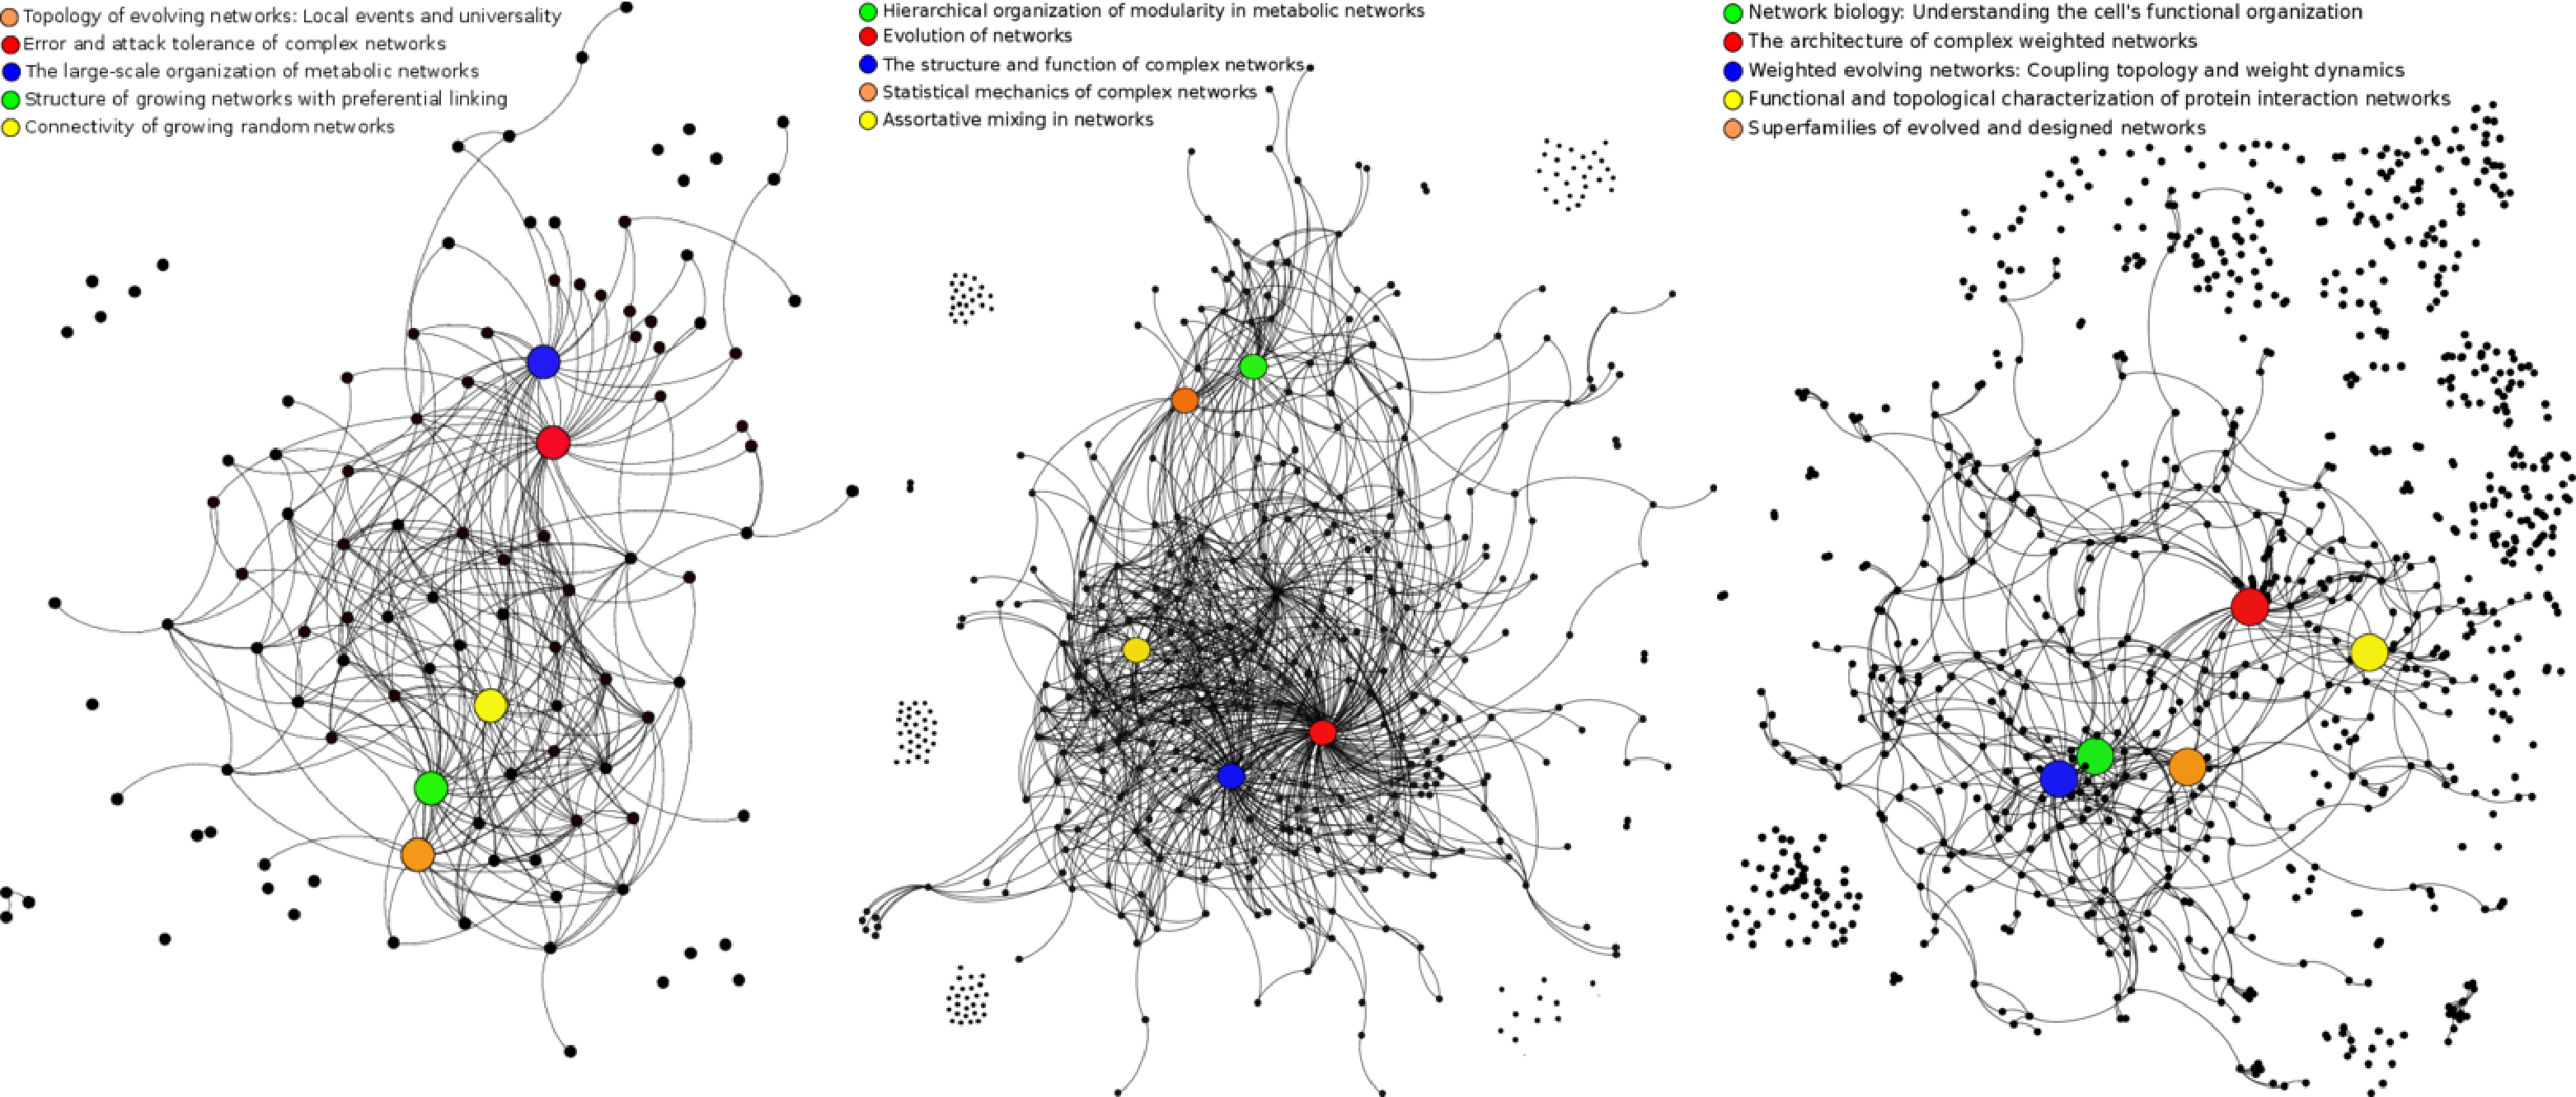
\includegraphics[width=\linewidth]{Figures/EN.pdf}

\caption{Ego-network for Barab\'asi and
R. Albert's  paper on scale-free networks \cite{Barabasi509}. We consider windows of size $w=2$ at $t$=1 (left), $t$=3 (center)
and $t$=5 (right), where $t$ is the number of years from
publication. Therefore the windows are non-overlapping and cover the
intervals 1-2, 3-4 and 5-6 (years after publication).
The EN is initially well connected, its link density is highest at
t=3, but it quickly becomes sparse, with a growing number of isolated
nodes. Some well known papers are highlighted with colors, their
titles are reported at the top. Figure adapted from Publication II.}
\label{fig:EN}
\end{figure}

While the EN approach aims at analyzing the local structure of the community around an idea/publication and its evolution in time, it is possible to
continue the analysis by "zooming out" gradually from the EN network, encompassing more and more layers of citations.
Even though a single paper might not have a massive first layer (i.e. citation count), it can accumulate a vast offspring in following layers, thus spreading its influence
to a large portion of the scientific network. 

The growth of the influence of an idea can be studied in its evolution, assigning a stronger weight to nodes
that lie in the lower circles and thus allowing to quantify the size and shape of the \textit{wake} of a paper \cite{10.1371/journal.pone.0113184}. Interestingly,
high values of this metric are able to reveal groundbreaking results that do not have high citation counts, with in particular Nobel laureates appearing as authors
of some of the most significant papers. In Publication IV we found a similar pattern: we introduced
a measure of the impact that a single paper has on the whole future corpus of science by allowing citing papers to "inherit" the scientific importance
of the cited paper. By recursively applying the method we are thus able to measure the global contribution of a paper in the scientific network and to compare the 
performance of papers between citations and impact. Fig. \ref{fig:nobel_impact} shows this comparison through a parameter $\delta = \frac{R_{c} - R_{i}}{R_{i}}$, where 
$R_{c}$ and $R_{i}$ are the rankings based on either citations (the former) or influence (the latter). $\delta$ measures
the outpferformance in impact vs. citation rankings, which is extremely high for Nobel papers if compared to papers with similar citation counts, thus
confirming that the cumulative importance "down the road" of scientific discoveries is not necessarily correlated to the first approximation, i.e.
the citation count.

\begin{figure}[h!]
\centering \large
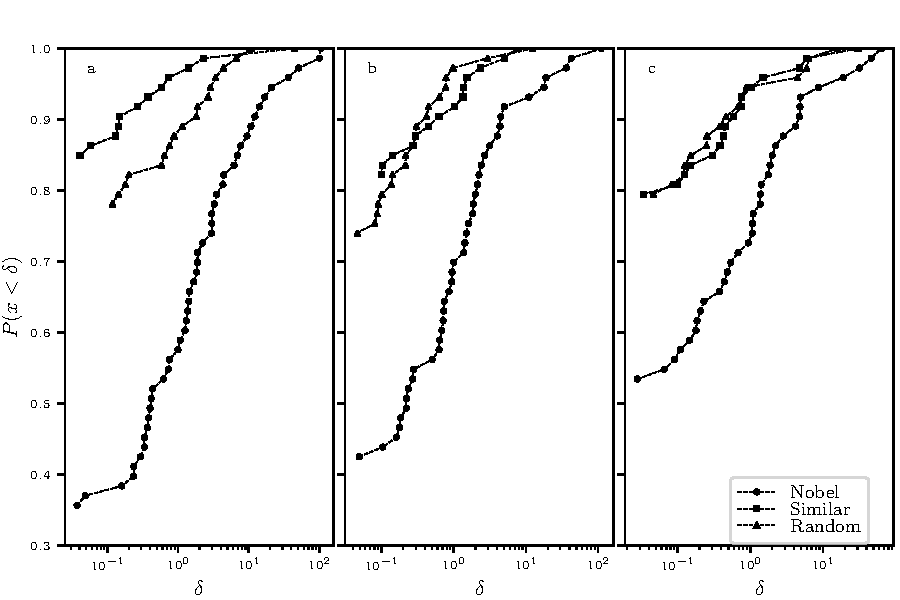
\includegraphics[width=.8\linewidth]{Figures/nobel_ranking_nCit.pdf}

\caption{Cumulative distribution of $\delta$ for Nobel papers, paper within a $3\%$ in citation volume in the same time interval compared to Nobel papers and for random papers
after five years (panel c), ten years (panel b) and at the end of the process in 2008 (panel a). Only papers
with positive $\delta$s are included. Nobel prize winning papers are more likely to climb the influence rankings, while similar papers behave
similarly to random papers. Also, while the fraction of Nobel papers that is climbing the ranking is increasing as time progresses, the control group
shows no significant change. Figure adapted from Publication IV.}
\label{fig:nobel_impact}
\end{figure}

As the previous examples show, the network structure of science can be an excellent indicator of the spread of ideas within the network. 
This kind of analysis has already been applied with success at a country and institutional
level \cite{Borner2006}. In this kind of framework, publications can be seen as new ideas introduced in a existing network, 
that are initially "exposed" to contagion from previous and become later the very source
of contagion for future works. This kind of approach borrowed from epidemiology \cite{Christakis2012}
is well known to be a driving force of the spread of new ideas \cite{Bettencourt2006513} and of the emergence and diffusion of topics across
disciplines. Susceptible-infected epidemic models applied to article networks
show that the diffusion of new ideas over disciplines takes a long time with the incubation period ranging from 4.0 to 15.5 years \cite{Kiss201074}. 

Another way to look at this process
is by comparison with genetics, seeing scientific ideas as genes that replicate/propagate themselves
to new publications in order to survive, an idea originally introduced by Dawkins in his book \textit{The Selfish Gene} \cite{selfishgene}. The term he coined
for these replicating entities is \textit{meme} and it has become extremely relevant nowadays, with the explosion of similar phenomena online that 
behave in such a way \cite{Leskovec:2009:MDN:1557019.1557077}. However, as genes and viruses replicate themselves to survive, they inevitably
end up competing for the same resources, thus leading to the inevitable disappearance of some of them \cite{Weng2012}. A meme based approach to
the spreading of scientific ideas has been attempted with success \cite{PhysRevX.4.041036}, introducing a meme score that quantifies the tendency of a 
scientific idea (e.g. chemical formulas or technical terms) to be replicated in a publication through a citation. Not surprisingly, high meme scores
are found to be important concepts in science.


\section{Communities, fields and multidisciplinarity}

In the previous sections we talked about the global structural properties of scientific networks that can be determined from network theory. However, the opposite process
can also be done. In the section on modularity and communities we discussed how the knowledge of the underlying structure of a network can be useful in order to devise methods
to analyze it, similarly in science we are aware \textit{a priori} that science is structurally organized in fields. Even within a single institution, there are separate
faculties or departments, in which scientists work separate one from another, with each group focusing on different branches of science. Fields are a concept everyone is familiar with
as the classical division of science in major branches such as Physics, Mathematics, Biology, Economics etc. is commonly used also outside the academic world and also
the ISI has a list of 21 static fields (or rather categories) used to label all journals. 

This categorization is simplistic and efficient on a superficial scale,
but we know science to be a intrinsically dynamic world. Bibliometric studies \cite{WeiweiCui2011} and studies on the co-occurrence network of scientific terms \cite{10.1371/journal.pone.0054847} have shown
that fields themselves are not static, but rather follow a life-cycle that may contain branching or merging events. It appears therefore evident from these observations that also
fields need to be studied not statically, but rather dynamically and that the information we know from scientific fields can be used recursively to analyze their changes
in time. 

Once again, works from epidemiology have been successfully applied to the topic. In a SEIR epidemic model scientists start off
being Susceptible to a new idea (i.e. working in a related field), transition to being Exposed to it (i.e. they have found out about it), proceed to become Infected spreading the idea before ultimately Retiring. 
Empirical evidence shows that the population growth of fields can be modeled with success by this 
model \cite{Bettencourt2008}. 

However, these processes are not always smooth: in 1970 the philosopher T. Kuhn discussed this matter in his famous book \textit{The Structure of Scientific Revolutions
} \cite{Kuhn:1970}, in which he described the process by which scientific knowledge progresses as being composed of periods of staticity separated by abrupt changes caused by \textit{paradigm
shifts} that challenge the scientific consensus. These shifts are mainly driven by discoveries of new information that contradicts and falsifies previous theories
and methods, thus requiring collaborative effort from the scientific community in order to provide new theoretical explanations. One of the most classic examples can be 
seen in the foundational crisis of most scientific fields at the end of the 19th century when Darwin's evolutionary theory, G{\"o}del's works on coherence and completeness and the new theory of Quanta
caused dramatic earthquakes in Biology, Mathematics and Physics. All these events happened sharply with either the experimental observation of new phenomena or the publication
of new innovative work which ultimately leads to completely new fields being born in a relative short time. 

One can therefore look at structural changes in the organization of fields
themselves in order to identify what are the crucial moments in the development of a single field. Studies on the temporal evolution of fields show that successful fields
grow in size, becoming more dense. In particular, the relationship between the number of edges and the number of nodes follows a scaling law :
edges = A(nodes)$^{\alpha}$, where $A$ and $\alpha$ are constant. This process is accompanied by a topological
transformation in the structure of the author network of the field: initially the authors are clustered in separate communities that, due to the densification
of the network, end up merging and forming of a \textit{large connected component} of authors, a phenomenon that does not take place for pathological cases (e.g. cold fusion in Physics)
due to the innovative failure of the original idea \cite{Bettencourt2009210}. This results show that the forming of a field is structurally connected to the forming of a sort of social network of authors
around an innovative concept. This social network, shown to be dense, can therefore be used as a \textit{ground truth} in community detection algorithms in order
to identify these communities in the global network. 

In fact, the changes in the connections between scientists and the subsequent change in modularity within the network
can be used to accurately model the birth of new fields as a process of merging and splitting of author communities \cite{Sun2013}. On the other hand, the diverse nature of fields
and their change in time undermines the possibility to use static definition of fields as a baseline for community detection. The application of modularity maximization
algorithm to paper network in fact has found that communities found in this way show a wide range of structure, varying from being strongly clustered to being barely noticeable \cite{Chen2010278}.
Furthermore, fields themselves are not monolithic blocks, but rather can be organized in structured hierarchical layers; Physics for example, manifests in its 
own paper network a number of subfields that have different local structure, with smaller subfields being more self-referential and thus more modular \cite{Sinatra2015}. This is to be expected:
the larger the extent of a field (or subfield), the more it is bound to see a diversification of its ideas and the reciprocal contamination with other fields and subfields. This process
leads to the birth of \textit{interdisciplinarity} and \textit{multidisciplinarity}.

The hierarchical nature  of fields and the structural overlapping across subfields and fields has led to the necessity to use also alternative methods for community detection, such
as clique percolation techniques \cite{Herrera2010}. Interdisciplinarity is not only an inevitable phenomenon of overlapping between fields,
but in recent years it has shown to become an intrinsic part of the core of Physics, gradually becoming more and more relevant \cite{Pan2012interdisciplinarity,Sinatra2015}.
Multidisciplainarity is slowly increasing and it can be analyzed in terms of the flow of information across fields \cite{Porter2009}, a technique that has led to the possibility of determining
the stabilization of interdisciplinary fields, thus becoming new stand alone disciplines \cite{10.1371/journal.pone.0008694}.

In Publication IV we studied the diffusion of scientific credit through the paper network, by spreading the scientific value of seed nodes from a field/subfield/journal of a certain year through the network.
By collecting the diffused scientific value and merging it into the same groups as the seed it is possible to measure the flow of information across fields. We found that
fields retain their information exponentially in time and that the exponent regulating the decay is increasing in time, thus manifesting an increase in multidisciplinarity which, 
however, might be a consequence of the increased rate of publication. A renormalization of time similar to the one in Publication I shows that the trend of increased interdisciplinarity is 
actually reversed, as shown in Fig.\ref{fig:multidisciplinarity}. Interestingly, multidisciplinarity shows to be the field slowing down the most in its tendency to share information, probably as a consequence
of it growing to the level of a stand-alone discipline with increased levels of self-referentiality.


\begin{figure}[h!]
\centering \large
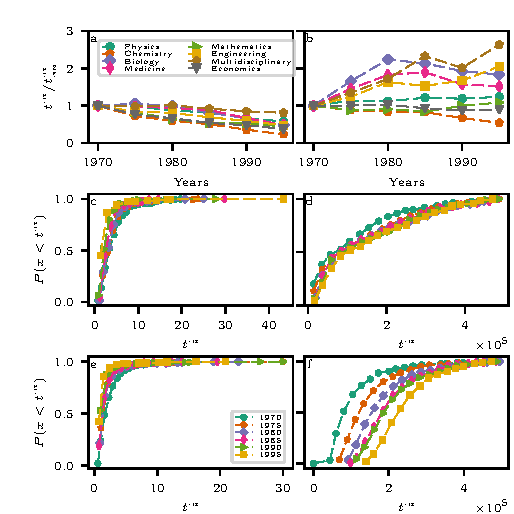
\includegraphics[width=.8\linewidth]{Figures/multidisciplinarity.pdf}

\caption{Changes in half life in time for the regular (left column, panels a-c-e) and renormalized scenario (panels b-d-f) and for different grouping of papers.
Panel a shows the evolution of the half life for a number of selected fields relatively to the 1970 value, in order to compare the trend across disciplines. We can see that fields
in general show a downward trend in which the half lives are decreasing. In panel b instead we can see the same evolution but but for the renormalized scenario, in which
time is measured in numbers of publications published. We can see that the trend either stabilizes or is reversed. Panels c and d shows the cumulative distribution of half lives for subfields and journals for 
different years, while panels e and f show the same distributions with renormalized half lives. We can see that the coloring order between the two columns is reversed, indicating
that also for subfields and journals are on average the same pattern as for the fields applies. Figure adapted from Publication IV.}
\label{fig:multidisciplinarity}
\end{figure}



\chapter{Science and Metrics}\label{Science and Metrics}

In 1955, Dr. Eugene Garfield published a fundamental paper in the history of bibliometric studies \cite{Garfield108}. In his work,
Garfield introduced the idea of a citation index, i.e., a database that would allow scientists to navigate the corpus of scientific publication through citation in order
to find valuable bibliographic material for their own research, an idea that eventually led to the foundation in 1960 of the Institute for Scientific Information (ISI).
While advocating for the importance of such index, Garfield used as an example the possibility to quantify the number of citations: \textit{"
Thus, in the case of a highly significant article, the citation index has a quantitative value, for it may help
the historian to measure the influence of the
article—that is, its ‘impact factor’"}, symbolically giving birth to the field of \textit{Scientometrics}, which
aims at providing a quantitative analysis of science and scientific research in general through statistical and mathematical analysis.
In 1972, Garfield
continued on this path by introducing a quantitative measure to rank journals based on their publication and citation count \cite{Garfield1972}. 

In its earliest
stages the field had a huge overlap with bibliometric and library studies in general, as well as with a quantitative analysis at a micro level, such as 
the individual habits of scientists \cite{069102832X}. With the increase of the availability of data scientometrics started to differentiate as its own
field aimed at the development of scientific indicators \cite{1208.4566}, also pushed by the increase need of instruments in the process of academic policy making 
\cite{doi:10.1080/09537329508524202}, with citation based measures being the dominating base in order to assess quality in scientific output. 
As more citation based analysis were being introduced \cite{Cole1972,vanRaan1993}, scientists also started to question the validity of such methods
to assess quality of research both from a technical point of view (i.e. the mathematical validity of the methods) as well as from a philosophical
one (do citations reflect quality?) \cite{ASI:ASI5,ASI:ASI7,MacRoberts1989,Seglen1997}.

In fact, the clash between the scientific requirement to cite relevant works along with the knowledge that metrics are used in order to assess
the quality of scientific research however, can lead to a vicious circle
in which the methods used to analyze the scientific outputs end up influencing the selection process of cited works \cite{HARGENS1990205}  or, in general, influencing the structure of 
Academia itself \cite{10.2307/765143}, thus compromising the previous underlying assumptions
of citations as a free and voluntary choice. In spite of these limitations, citation based metrics continued being introduced and citation based
rankings were introduced for authors \cite{10.2307/4152261} as well as for universities \cite{RankingUni}. In this chapter I will briefly go
through some of the most popular ranking measures for individual papers and authors.





\section{Publication rankings}
Even though a large of number of rankings for authors and journals were being developed, paper rankings required more time to be introduced.
Unlike metrics meant for groups of papers that allow to address the rankings statistically, ranking of papers comes down to the ranking
of individual nodes in a network. This task can be extremely challenging in the scientific network, especially considering
the difference in citation patterns across fields both quantitatively \cite{Radicchi11112008} and conceptually \cite{Franceschet2010}. Therefore
citation counts remained for a long time a valid ranking method locally, provided that one would know what the typical citation count
of a paper on a topic could be. 

In order to allow for a fair ranking across \textit{all} scientific publications instead, one would have to put into context the local properties of a paper, i.e.
 the community from which the citations come, with the global properties of the network, i.e. how the single community relates to all the others. This problem
 is closely related to what the well known Page Rank (PR) algorithm of Google does \cite{Page99thepagerank}. Page Rank was the most successful method among a number
 of solutions introduced in the 90s \cite{Kleinberg1999} for solving the problem of rating Web Pages in the WWW. Curiously, in their paper,
 Page and Brin analyze comparison between ranking pages and publications, concluding that citation counts are a far too limited tool in the presence
 of a large evolving network.
 
 The idea behind PR is to provide a metric for quality of web pages that takes into account the quality of the citations 
 themselves. In this framework therefore, a large degree (the equivalent of citation count) cannot be enough to receive a high PR as these citations
 might be incoming from poorly ranked nodes. In this framework therefore quality is built among a reinforcing behavior in which high quality pages
 "support" each other ranking wise through mutual citations or, in general, by being highly connected within the same community. Mathematically, the PR
 algorithm can be implemented in many ways, among which a recursive method that initially assigns equal ranking to all papers and then proceeds
 to propagate the ranking through the equation:
 \begin{equation} \label{eq:PR}
 PR(j) = \frac{1 -d }{N} + d \sum_{j \in N_{i}} \frac{PR(j)}{|N_{j}|} 
 \end{equation}
 where $N$ is the total number of nodes and $N_{i}$ is the neighborhood of node $i$. The PR can also be thus calculated by solving the eigenvalue equation $\vec{R} =  (1 -d)/N \vec{1} + d A\vec{R}$ where $\vec{R}$ is the array ranking and $A$ is the adjacency matrix of the WWW. The possibility 
 to express the PR algorithm in the solving of an eigenvalue equations shows that the PR is ultimately a centrality measure. The problem can be solved efficiently with the power method, requiring ~52 iterations to obtain convergence for the 
snapshot of the WWW that Page and Bring used in 1999 \cite{Page99thepagerank}.
The parameter $d$ is a quantity called \textit{damping factor} and it plays a crucial factor in the algorithm. The damping factor is linked to the
implementation of the model as a random walker that propagates the PR of a single node by randomly jumping
  to a nearby one through its links. In this context, the damping factor represents the probability for the walker to "get bored", as the authors say, and jump to a random
 node in the network after $1/d$ steps on average. Practically, this factor prevents the influence of "sinks" (node or group of nodes without outgoing links) that would absorb all 
 the rankings; with
 $d = 1$ we would have an infinite series of clicks, thus allowing the walker to be trapped in such sinks, while $d=0$ would be equal to a situation
 in which the PR are uniform and constant. However, the damping factor also plays a fundamental role in the correct renormalization of scores across communities
 of different sizes  \cite{Xie2007}. If a community is strongly isolated from the core of the network (i.e. it has few incoming links), it might be difficult
 for the random walker to enter the community and to correctly evaluate its global PR, without the necessity to perform separate rankings.
 
 This 
 feature of the Page Rank thus allows to solve issues linked to different topological structures of scientific communities in citation networks both across fields and within fields \cite{Maslov2008}.
 In 2007 two papers attempted two adapt the Page Rank algorithm to scientific publications. Chen et al. applied the pure Page Rank algorithm to all 
 publications belonging to the Physical Review family of journals from 1893 to 2003, with a choice of $d=0.5$ as they believed it would better
 reflect the citation practices in science. Even though the PR was shown to be positively correlated with the citation count, as expected  \cite{Fortunato:2007:API:1422841.1422847},
 a few paper were shown to be significant outliers and were identified as being important "gems" in Physics. In the same years a follow up paper came that introduced
 the CiteRank algorithm \cite{Walker2007}: a generalization of the PR algorithm, in which the effects of aging into the Page Rank algorithm
 are taken into account. This was necessary as the PR has in intrinsic directionality based on the fact that papers
 cannot be cited by older ones, thus forcing the "flow" of the PR towards older entries. In the CR framework, the random walker starts from a \textit{recent} paper
 and recursively follows scientific papers selecting a link not randomly, but rather in a weighed process that penalizes older papers and therefore
 gives a stronger value to novelty.
 
In Publication IV we introduced a measure that we called \textit{persistent influence}. Despite appearing at first glance similar to PR methods, it is conceptually
very different. In our approach in fact, we reversed the flow of time and we turned a stochastic process into a deterministic one. While the PR methods
measure how likely a random walker is to land on a single node, we imagined a scenario in which the knowledge created in an article percolates through the network of articles.
In this framework citing papers do not pass their own credit to the cited papers, but rather inherits it \textit{from} them.
Mathematically, we start from an original seed $s$ with an initial influence $I_s=1$ and we allow newer papers to inherit the influence
through the equation :
\begin{equation} \label{eq:impact}
 I_{j} = \sum_{i \in N_{j}}  \frac{I_{i}}{ k_{j}^{in}}
\end{equation}
where $ k_{j}^{in}$ is the in-degree (or, number of references) of the article $j$, and $N_j$ is the set of out-neighbors. The normalization guarantees that the total influence
that the cited articles have on article $j$ is 
constant and that the influence value does not exceed $1$.
As the process continues, the influence values dilute through the network, but at the same time they are spread to increasing number of articles. At the end of the process
we can then proceed to observe the influence that a single paper has had on the whole scientific network as shown in Fig.\ref{fig:influence}.





 \begin{figure}[h]
\centering
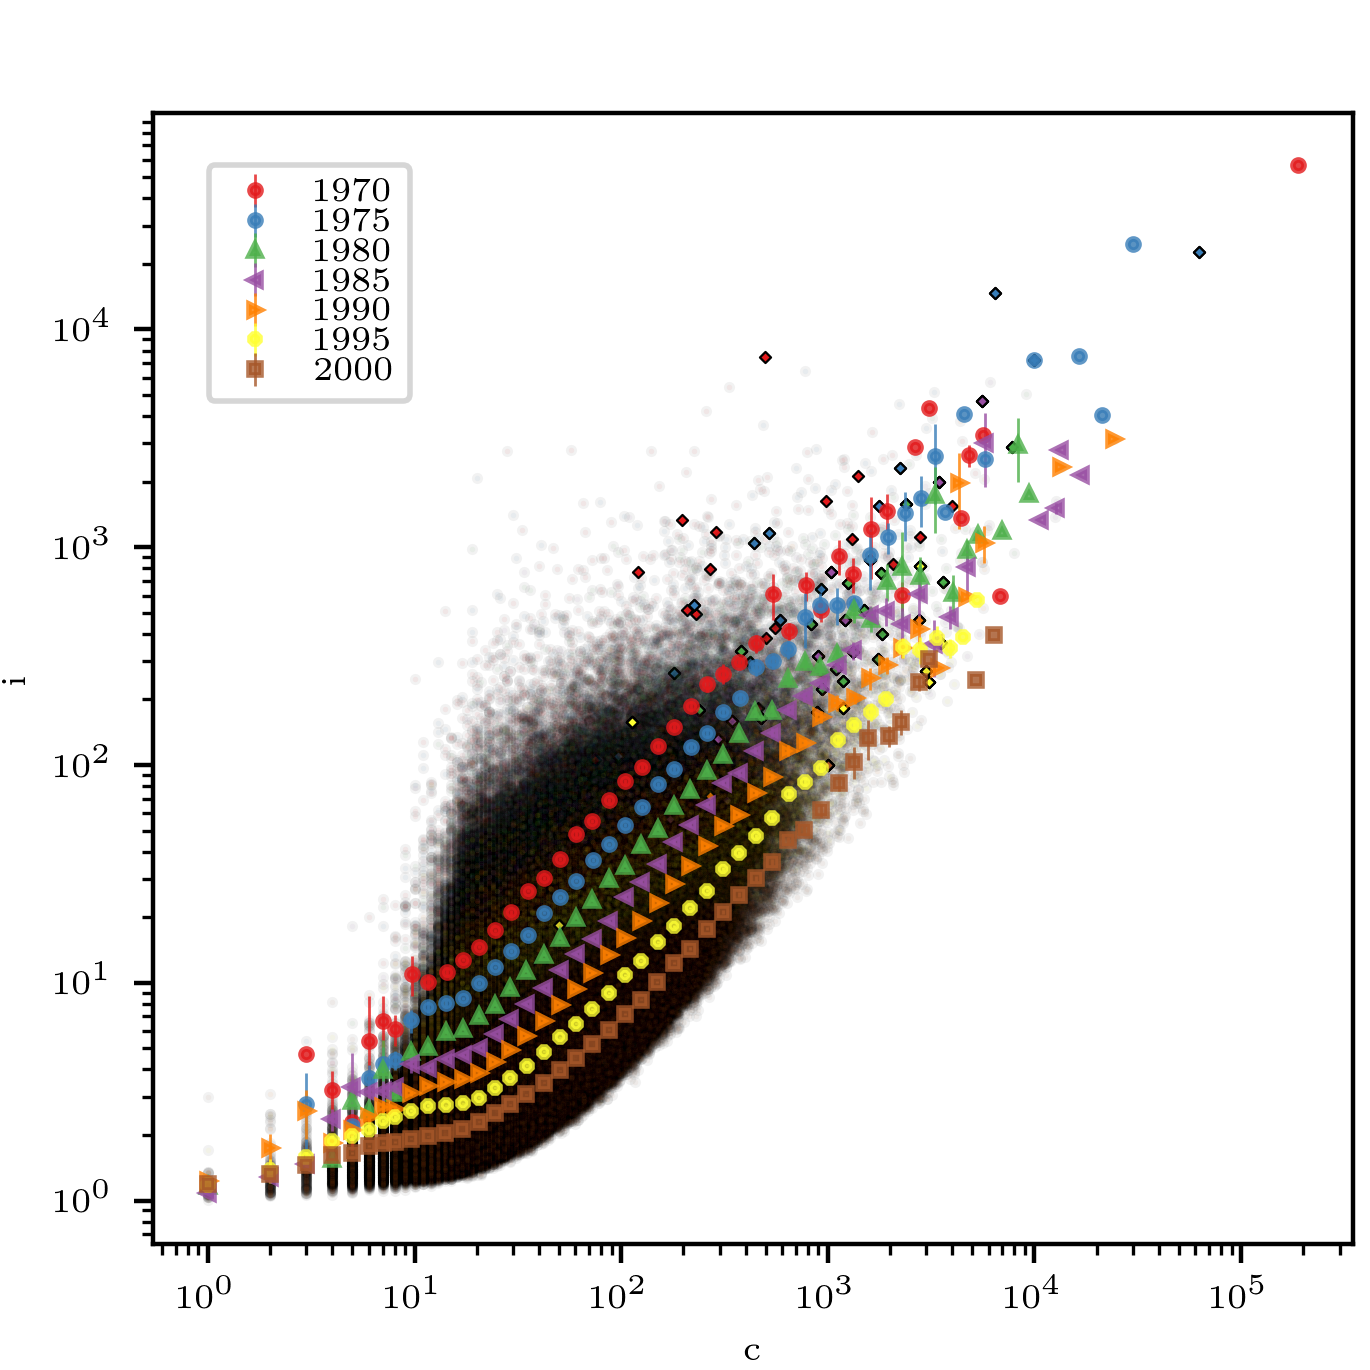
\includegraphics[width=.8\textwidth]{impact_thesis.png}%
\caption{Scatter plot of values for citations vs persistent influence for different years. The full dots represent the average influence for publications within the same citation
bin. Diamond shaped dots represent individual Nobel prize winning papers, the coloring of which is assigned according to the closest year to the publication date. The values appear to be correlated by a power law curve, but within
each citation bin influence values can span multiple orders of magnitude. Also, Nobel prize winning papers are clustered in the top right corner, indicating
both a high citation count and high influence values. Figure adapted from publication IV.}
\label{fig:influence}
\end{figure}


\section{Author rankings}

Science has primarily been a public endeavor carried out in public universities. 
As more investments were being
put into research, it is no surprise that soon pressure to properly quantify scientific output would start to increase \cite{Lane2011}.
Citation counts served this purposes and have been used to decide how to allocate funds \cite{Bornmann2005} as well as to select candidates for
academic positions \cite{Boyack2003}. In this search for a "perfect" measure, one of the most important contributions was developed in 2005 by J.E. Hirsch \cite{10.2307/4152261},
who introduced for the first time a clear metric aimed at ranking scientists through their citation count.
The h-index is based on a very straightforward definition: an author has index $h$ if $h$ of their publications have gathered at least $h$ citations each and the remaining
papers have citations $\leq h$. 

The new metric became immediately popular among scientists and started being considered as a standard to which to compare standard bibliometric indicators  \cite{vanRaan2006}, both
thanks to its simplicity and its ability to "rescue from obscurity" scientists who had been heavily contributing in very specific fields \cite{Ball2005}. However,
the h index was also soon discussed from a methodological point of view as authors claimed that it was not a correct way to quantify a career. In particular, it was pointed
out that one can artificially alter one's index through self-citations \cite{PURVIS2006} and that
citations need to be weighed, as not all of them carry the same weight \cite{Wendl2007}. As other critiques followed, tackling the limitation of the h index in guaranteeing a fair
ranking of scientists, new methods appeared, trying to fix the structural limitations of the h-index: indexes focusing on high cited papers (g-index) \cite{Egghe2006}, indexes focusing
on the average citations of the papers that grant the h-index to an author (A and AR index) \cite{Jin2007}, indexes focusing on the different
volume of publications across authors (h-normalized index) \cite{Sidiropoulos2007}, indexes that take into account the difference in lengths in careers (m-quotient) \cite{Burrell2007},
indexes that focus only on the most cited papers (Google Scholar's \textit{i10} index) \cite{i10} and many others \cite{Alonso2009}.

As citation based indexes continued to proliferate however, another key aspect became important to tackle: what is the predictive power of the h index? Since these measures
were being actively used as proxies of scientific excellence in the hiring process, it is normal to investigate the ability of the h index to predict the quality of individual
careers. Hirsch himself soon tackled the aspect, reporting that the h index is able to predict a carreer: \textit{"That is, a researcher with a high h index after 12 years is highly
likely to have a high h index after $24$ years"}\cite{Hirsch2007}.  
While more works have similar results by combining the h index with other citation based metrics \cite{Acuna2012}, other publications reported a different scenario in which
past citations are only good at predicting future citations to \textit{past} publications, but are ultimately not good at predicting future citations to \textit{future} publications \cite{Mazloumian2012}.
This contrast  between prediction of previous results vs prediction of past results brought back the attention to the
validity of the h index as a measure to predict the evolution of a career. In fact it has been argued that 
the h index suffers from methodological flaws due to the nature of its definition: the h index is a non stationary measure \cite{Penner2013b} which has a high auto correlation 
to its whole previous history, ultimately causing the h index being a good predictor of \textit{itself} \cite{Schreiber2013}. Quantitatively, any cumulative, non decreasing
measure has auto correlation between its index at two different stages of the career following the relation $Cor(h(t),h(t + \Delta t)) = \sqrt{\frac{t}{t + \Delta t}}$, which means
that the predictive power of such indexes is much lower when trying to estimate an individual's h-index many more years into their future than the current career
academic age ($t/(t + \Delta t) \rightarrow 0$) and that for the same prediction interval ($\Delta t$) the prediction will be much more sound for a senior researcher rather
than for a junior one \cite{Penner2013}. This latter result leads to the consequence that the h index of a researcher, as their career progresses, increases regardless
of their productivity \cite{Schreiber2013}. 

These findings are
 ultimately in contrast with the very idea that metrics should be used to hire someone for that they will do, since such kind of citation metrics based on previous results appear to be able
 grasp mainly only what a scientist has done and show their strongest predictive limitations for the cases in which these will be used in real academic hiring decisions \cite{Penner2013}. Furthermore,
 it can even introduce a self-reassurance bias as bureaucrats may actually take advantage of the metric auto correlation in order to have a guarantee that metrics will increase \cite{Schreiber2013}.

 In parallel to citation based rankings however, other authors have attempted to introduce rankings based on methods similar to the Page Rank algorithm discussed in the previous paragraph \cite{PhysRevE.80.056103,Yan2010}
as well as on centrality measures similar to the one mentioned in section \ref{sec:centrality} \cite{Yan2009}, but ultimately the intrinsic feasibility of the distinction
between quality and quantity in scientific output is still an open question \cite{Kaur2015} and the predictability of individual indexes remains a statistical method that can possibly
lead to average results, while careers have been shown to be extremely uncertain and volatile, with single events leading both to sudden career boosts \cite{10.1371/journal.pone.0018975} and negative shocks
to equally extreme, yet opposite consequences \cite{Petersen2012}. Even though it is probably impossible to either develop a perfectly universal and unbiased metrics or to
prevent the usage of metrics in the academic selection process, it has been argued that it would be most beneficial to minimize the increasing ``taste for publication'' \cite{Osterloh2010}
that has been gradually replacing the "taste for science" and to rely on multiple factors and measure instead of reducing the process to the evaluation of a 
single statistic \cite{Frey2010}.
\chapter{Scientific Results and Discussion} \label{Results and Discussion}

\section{Temporal patterns}

Publication I studies the changes over time of the age statistics in the awarding of Nobel Prizes. In the early days of the award, prizes in Physics, Medicine and Chemistry had
a $\approx 50\% $ chance to be awarded to discoveries from the previous decade, while only a smaller fraction $\approx 20\%$ of prizes was awarded to discoveries older than 20 years. In time
the pattern has dramatically reversed, with nowadays more than half of the prizes being awarded over 20 years from discovery. As a result, also the age at which the Nobel prize
laureates are awarded has seen a drastic increasing trend, that ultimately might lead, by the end of the century, to not be able to reward an old discovery, since the prizes cannot
be awarded posthumously. While it is not simple to offer an exhaustive explanation for this trend, we suggested that a plausible one might be one of two extreme scenarios:
on one hand it could be possible that the number of groundbreaking discoveries has been decreasing, therefore forcing the Nobel committee to look at older ones to find a worthy winner;
on the other hand, it could be that the rate of new significant discoveries has increased so much that the limit to only 2 independent discoveries being awarded every year cannot
keep up with the pace of scientific innovation. 

Publication II studies the intrinsic temporal features of the life cycle of an individual paper. Publications from a dataset of over 50 million papers and 600 million
citations were grouped by peak year, i.e. the year in which the higher number of yearly citations was reached, thus separating the history of a paper between its rise to
"fame" and its consequent decay. In order to compare individual cycles, citation cycles were renormalized so that the maximum value (i.e. the peak) would equal to one. The time required
to peak has been constantly shrinking in time across the fields of Physics, Medicine, Biology and Chemistry, with Biology showing the lowest numbers in general. The result is coherent
with previous studies that show the average reference age being increasing in time, thus allowing to allocate less attention to more recent papers, which inevitably peak earlier. On the other
side of the peak, the decay was found to have a form very close to either an exponential or a power law, with the former working better for older publications and the latter
being a better fit as time goes by. We explained this feature as a consequence of the citation mechanism being linked to a ultradiffusive process, i.e. a mechanism in which a later event might be caused by or correlated to an earlier event
or a combination of earlier events: in this case the citation count. This ultradiffusive approach allows to quantify the probability of a paper having a certain number 
of citations as an auto correlation function between citation counts, which can be shown analytically to be either exponential or power law in its form, as it was found in the data. Finally
a non-parametric quantification of the time required to decay (i.e. an half life) allows us to show a similar pattern as for the time to peak: across fields there is a clear
shrinking in the time required for a paper to be forgotten. 

Publication III studies the temporal evolution of the Ego Network of highly cited scientific papers. An Ego Network built based on a single paper (the EGO) and is formed
by the publications citing as nodes (the Ego is not included) with all the citations between such publications as edges. Since results of Publications I have shown
that the cycle of a paper is extremely short, the EN was analyzed in its evolution in snapshots of 2 and 3 years in size, thus focusing on a temporally coherent bulk of papers that shared
the Ego in their reference lists. The structure of the EN in its earliest years initially consolidates in a dense community, but is later followed by a consistent
scenario, in which the networks fragment into many small components within 10 years from publication of the
ego-paper, possibly linked to a specialization of the offspring of the Ego or to an increased popularity of the ego across disciplines, thus affecting the probability of cross citing.

\section{Cumulative patterns}

Publication IV studies the cumulative process of knowledge spreading stemming from the knowledge created by an individual papers. Starting from individual papers a measure
called persistent influence is introduced and is
based on citing papers inheriting the knowledge of cited papers. The process is then repeated recursively, thus propagating the initial influence into a cascade that eventually allows to quantify
the overall influence a single paper has had on the whole corpus of scientific publications, unlike citation counts, which are based only on a local snapshot of the network limited
to the first "round" of citations. Nobel winning papers are used as a benchmark for highly influential papers and in the persistent influence framework are found to be performing
significantly better in their influence measures if compared to papers with similar citation counts, thus reinforcing the idea that a difference exists between local and global influence
of a paper. 

Publication IV also introduced a diffusive method that is used to quantify the flow of knowledge across categories (field,subfields and journals). Curves representing the loss of knowledge to other
scientific categories shows a constant pattern where knowledge rapidly falls and then converges to a plateau in a typical time (the half life). While the plateau value varies across disciplines but is constant in time,
the half life is decreasing in time for virtually all fields, suggesting an increase in interdisciplinarity. Furthermore, there seems to be in time a narrowing of the difference in
half lives of humanistic fields (higher values) and of hard sciences (lower values), possibly linked to a structural change in the citing patterns of humanities. Multidisciplinary studies
are found to have a peculiar pattern: their plateau value is increasing and their half life slowing down is among the slowest, suggesting that multidisciplinarity is possibly
becoming a stand alone field that is growing internally.

Publications II and IV offer a tool of renormalization that uses cumulative information to rescale temporal patterns, thus connecting the two aspects. In both studies, temporal patterns
were calculated using years as an absolute measure of time. However, in both cases, the quantities being measured were part of a system in which "updates" happen every time a new publication
appears. In a system where publications come in at a constant rate, the two measures would coincide but that is not the case in science, where publications are growing at a slow,
yet exponential rate. A renormalization of the time based on the number of publications instead, offers a dramatic change in the patterns observed. The speeding up in the 
half life for the decay of attention of a paper shown in Publication I slows down to the point where the process seems to be stable over decades and across fields, thus providing evidence
for the fact that a faster decay is just a consequence of the impossibility for scientists to keep track for the ever growing amount of published material. Similarly,
the speeding up of the spread of knowledge across fields found in Publication IV also changes its structure, indicating that the increasing speed of knowledge sharing across scientific fields
could be explained by the increase in the speed at which the system is updated.


\clearpage
\section{Discussion}
Science of science as a field has seen a massive series of changes in the time since its formulation in the post war period. For a long time the pursuit of new findings in the field
was hindered by the absence of properly indexed data sets that would allow a systematic analysis of the data available. As scientific data piled up over the decades and with
the ever growing role of digitalization in modern times, such hinders were removed, uncovering a massive amount of information on the underlying dynamics that 
govern the way science works and operates.

Ever since an increasing amount of effort has been put into the uncovering of the patterns hidden in data from scientific publications: connections between papers, authors,
institutions, fields, countries allowed to unravel the intrinsic properties that are at the basis of the production of scientific material. In this kind of research the basic
approach has often been the one to analyze the data in locally and temporally confined snapshots. Furthermore, as scientific research sees its economical aspects become more relevant year after year, quantification of scientific output has also seen a spark in interest both from scientists
and from those hiring them. This has led to a constant search for perfect metrics able to grasp universal properties for individual authors,journals or papers, compacting longitudinal careers, both past and future,
into a mere number.

The research presented in this Thesis presents a diametrically opposed point of view to the matter; science does not represent a static platform for the output 
of new information, but is rather an ever changing
system with sociological, economical and geographical characteristics, which is bound to be influenced by the constant modification of the real world on which it is ultimately based. Such changes in turn, lead to a modification of science's very own
structure, thus creating patterns that are constantly evolving in time. In particular, science has been going through a constant exponential growth over the decades
since the post war era, with more and more scientific knowledge accumulating on top of previous findings over a short interval of time. 

The main focus of this Thesis has been to analyze these temporal and cumulative patterns both by considering their individual contribution to the analysis of scientific
data as well as their united one. Only with this \textit{combined} approach has it been possible to properly quantify the dynamics of life cycles of citation histories and Ego Network
structures of individual papers, as well as the information flow between areas of science. Similarly, it allowed to introduce a paper-based measure to quantify the influence of a single 
publication over the whole corpus of scientific data, also allowing to track its evolution in time.


\renewcommand{\bibname}{References}
\bibliographystyle{ieeetr}
\bibliography{references.bib}


\addpublication{Francesco Becattini, Arnab Chatterjee, Santo Fortunato, Marija Mitrović, Raj Kumar Pan, Pietro Della Briotta Parolo}{The Nobel Prize delay
}{Physics Today}{DOI:10.1063/PT.5.2012}{May}{2014}{Copyright Holder}{j1}
\addpublicationpdf{articlespdf/nobel_PT.pdf}
\addcontribution{The author contributed to the collection of the data.}

\addpublication{Pietro Della Briotta Parolo, Raj Kumar Pan, Rumi Ghosh Bernardo A. Huberman, Kimmo Kaski, Santo Fortunato}{Attention Decay in Sciene}
{Journal of Informetrics}{
Volume 9, Issue 4,  Pages 734–745}{October}{2015}{Copyright Holder}{j1}
\addpublicationpdf{articlespdf/attention_decay.pdf}
\addcontribution{The author carried out most of the analysis. Primary writer of the article.}

\addpublication{Pietro Della Briotta Parolo, Santo Fortunato}{Uncovering the Dynamics of Ego Networks of Scientific Gems}{preprint}{
submitted to peer review}{January}{2017}{Copyright Holder}{j1}
\addpublicationpdf{articlespdf/EgoNetworks.pdf}
\addcontribution{The author implemented the analysis. Major role in writing the article.}

\addpublication{Pietro Della Briotta Parolo, Mikko Kivel\"a, Kimmo Kaski}{On the Shoulders of Giants: tracking the cumulative knowledge spreading in citation
networks}
{preprint}{
submitted to peer review}{June}{2017}{Copyright Holder}{j1}
\addpublicationpdf{articlespdf/SOG.pdf}
\addcontribution{The author implemented the analysis. Major role in writing the article.}
\end{document}


